
%%%%%%%%%%%%%%%%%%%%%%%%%%%%%%%%%%%%%%%%%%%%%%%%%%%%%%%%%%%%%%%%%%%%%%%%%%%%%%
%                                                                            %
%  ************************** AVISO IMPORTANTE **************************    %
%                                                                            %
% Éste es un documento de ayuda para los autores que deseen enviar           %
% trabajos para su consideración en el Boletín de la Asociación Argentina    %
% de Astronomía.                                                             %
%                                                                            %
% Los comentarios en este archivo contienen instrucciones sobre el formato   %
% obligatorio del mismo que complementan los instructivos web y PDF.         %
% Por favor léalos.                                                          %
%                                                                            %
% No deben borrarse los comentarios en este archivo. En caso contrario,      %
% el sistema de recepción de manuscritos no permitirá el envío de su         %
% contribución. No se permite el uso de \newcommand ni definiciones          %
% particulares de cada autor.                                                %
%                                                                            %
%%%%%%%%%%%%%%%%%%%%%%%%%%%%%%%%%%%%%%%%%%%%%%%%%%%%%%%%%%%%%%%%%%%%%%%%%%%%%%

%%%%%%%%%%%%%%%%%%%%%%%%%%%%%%%%%%%%%%%%%%%%%%%%%%%%%%%%%%%%%%%%%%%%%%%%%%%%%%
%                                                                            %
%  ************************** IMPORTANT NOTICE **************************    %
%                                                                            %
%  This is a help file for authors who are preparing manuscripts to be       %
%  considered for publication in the Boletín de la Asociación Argentina      %
%  de Astronomía.                                                            %
%                                                                            %
%  The comments in this file give instructions about the manuscripts'        %
%  mandatory format that complement the instructions distributed as a PDF    %
%  and findable in the BAAA web. Please read them.                           %
%                                                                            %
%  The comments in this file must not be deleted. Otherwise, your            %
%  contribution will be rejected by the manuscript reception system.         %
%  The use of \newcommand and author definitions are forbidden.              %
%                                                                            %
%%%%%%%%%%%%%%%%%%%%%%%%%%%%%%%%%%%%%%%%%%%%%%%%%%%%%%%%%%%%%%%%%%%%%%%%%%%%%%

\documentclass[baaa]{baaa}

\usepackage[pdftex]{hyperref}
\usepackage{subfigure}
\usepackage{natbib}
\usepackage{helvet,soul}
\usepackage[font=small]{caption}

%%%%%%%%%%%%%%%%%%%%%%%%%%%%%%%%%%%%%%%%%%%%%%%%%%%%%%%%%%%%%%%%%%%%%%%%%%%%%%
%                                                                            %
%  Seleccione el idioma de su contribución: Recuerde que todos los           %
%  componentes del documento (titulo, texto, figuras, tablas, etc.)          %
%  deben estar en el mismo idioma.                                           %
%                                                                            %
%  Select the language of your contribution: Please remember that all       %
%  document parts (title, text, figures, tables, etc.) must be in the        %
%  same language.                                                            %
%                                                                            %
%  0: Castellano / Spanish                                                   %
%  1: Inglés / English                                                       %
%                                                                            %
%%%%%%%%%%%%%%%%%%%%%%%%%%%%%%%%%%%%%%%%%%%%%%%%%%%%%%%%%%%%%%%%%%%%%%%%%%%%%%

\contriblanguage{0}

%%%%%%%%%%%%%%%%%%%%%%%%%%%%%%%%%%%%%%%%%%%%%%%%%%%%%%%%%%%%%%%%%%%%%%%%%%%%%%
%                                                                            %
%  Seleccione el tipo de contribución solicitada:                            %
%                                                                            %
%  Select the requested contribution type:                                   %
%                                                                            %
%  1: Presentación mural / Poster                                            %
%  2: Presentación oral / Oral contribution                                  %
%  3: Informe invitado / Invited report                                      %
%  4: Mesa redonda / Round table                                             %
%  5: Presentación Premio Varsavsky / Varsavsky Prize contribution           %
%  6: Presentación Premio Sahade / Sahade Prize contribution                 %
%  7: Presentación Premio Sérsic / Sérsic Prize contribution                 %
%                                                                            %
%%%%%%%%%%%%%%%%%%%%%%%%%%%%%%%%%%%%%%%%%%%%%%%%%%%%%%%%%%%%%%%%%%%%%%%%%%%%%%

\contribtype{2}

%%%%%%%%%%%%%%%%%%%%%%%%%%%%%%%%%%%%%%%%%%%%%%%%%%%%%%%%%%%%%%%%%%%%%%%%%%%%%%
%                                                                            %
%  Seleccione el área temática de su contribución:                           %
%                                                                            %
%  Select the thematic area of your contribution:                            %
%                                                                            %
%  1 [AEC]:   Astrofísica Extragaláctica y Cosmología /                      %
%             Extragalactic Astrophysics and Cosmology                       %
%  2 [EG]:    Estructura Galáctica / Galactic Structure                      %
%  3 [AE]:    Astrofísica Estelar / Stellar Astrophysics                     %
%  4 [SE]:    Sistemas Estelares / Stellar Systems                           %
%  5 [ICSA]:  Instrumentación y Caracterización de Sitios Astronómicos /     %
%             Instrumentation and Astronomical Site Characterization         %
%  6 [MI]:    Medio Interestelar / Interstellar Medium                       %
%  7 [OCPAE]: Objetos Compactos y Procesos de Altas Energías /               %
%             Compact Objetcs and High-Energy Processes                      %
%  8 [SH]:    Sol y Heliosfera / Sun and Heliosphere                         %
%  9 [SSE]:   Sistemas Solar y Extrasolares / Solar and Extrasolar Systems   %
% 10 [HEDA]:  Historia, Enseñanza y Divulgación de la Astronomía /           %
%             History, Teaching and Spreading of Astronomy                   %
% 11 [O]:     Otros / Other Topics                                           %
%                                                                            %
%%%%%%%%%%%%%%%%%%%%%%%%%%%%%%%%%%%%%%%%%%%%%%%%%%%%%%%%%%%%%%%%%%%%%%%%%%%%%%

\thematicarea{8}

\title{Estudio de Validación Tomográfica del Modelo MHD AWSoM}
%\subtitle{Instrucciones de estilo}

%%%%%%%%%%%%%%%%%%%%%%%%%%%%%%%%%%%%%%%%%%%%%%%%%%%%%%%%%%%%%%%%%%%%%%%%%%%%%%
%                                                                            %
%  Agregue un título corto para el encabezado de las páginas pares.          %
%                                                                            %
%  Add a short title to appear in the header of even pages.                  %
%                                                                            %
%%%%%%%%%%%%%%%%%%%%%%%%%%%%%%%%%%%%%%%%%%%%%%%%%%%%%%%%%%%%%%%%%%%%%%%%%%%%%%

\titlerunning{Validación Modelo AWSoM}

%%%%%%%%%%%%%%%%%%%%%%%%%%%%%%%%%%%%%%%%%%%%%%%%%%%%%%%%%%%%%%%%%%%%%%%%%%%%%%
%                                                                            %
%  Lista de autores. Los nombres de los autores deben estar separados por    %
%  comas, y deben tener el formato A.E. Autor (iniciales apellido(s); sin    %
%  coma entre apellido e iniciales ni espacios entre las iniciales).         %
%                                                                            %
%  Author list. Authors' names must be separated by commas, and stick to     %
%  the format A.E. Author (initials Family name -neither commas between      %
%  name and the initials nor blanks between the initials).                   %
%                                                                            %
%%%%%%%%%%%%%%%%%%%%%%%%%%%%%%%%%%%%%%%%%%%%%%%%%%%%%%%%%%%%%%%%%%%%%%%%%%%%%%

\author{D.G. Lloveras\inst{1}, A.M. Vásquez\inst{1}, F.A. Nuevo\inst{1}, C. Mac Cormack\inst{1}, N. Sachdeva\inst{2},\\ W. Manchester IV\inst{2}, B. Van der Holst\inst{2}, \& R.A. Frazin\inst{2}}
\authorrunning{Lloveras et al.}


%%%%%%%%%%%%%%%%%%%%%%%%%%%%%%%%%%%%%%%%%%%%%%%%%%%%%%%%%%%%%%%%%%%%%%%%%%%%%%
%                                                                            %
% Por favor provea una dirección de e-mail de contacto para los lectores.    %
%                                                                            %
% Please provide a contact e-mail address for the readers.                   %
%                                                                            %
%%%%%%%%%%%%%%%%%%%%%%%%%%%%%%%%%%%%%%%%%%%%%%%%%%%%%%%%%%%%%%%%%%%%%%%%%%%%%%

\contact{dlloveras@iafe.uba.ar}

\institute{
Insituto de Astronomía y Física del Espacio, CONICET--UBA, Argentina \and
Climate and Space Sciences and Engineering, Universidad de Michigan, EEUU.
}

%%%%%%%%%%%%%%%%%%%%%%%%%%%%%%%%%%%%%%%%%%%%%%%%%%%%%%%%%%%%%%%%%%%%%%%%%%%%%%
%                                                                            %
%  El resumen y el abstract son ambos obligatorios, independientemente del   %
%  lenguaje elegido.                                                         %
%                                                                            %
%  The Resumen and the abstract are both mandatory, regardless of the chosen %
%  language.                                                                 %
%                                                                            %
%%%%%%%%%%%%%%%%%%%%%%%%%%%%%%%%%%%%%%%%%%%%%%%%%%%%%%%%%%%%%%%%%%%%%%%%%%%%%%

\resumen{
Los modelos magnetohidrodinámicos (MHD) tridimensionales (3D) de la corona solar, necesarios para modelar y predecir el clima espacial, deben ser validados observacionalmente. A escala global, esto puede ser hecho mediante tomografía de medida de emisión diferencial (DEMT), que provee resultados 3D de densidad y temperatura electrónica en la baja corona ($1.0-1.25 \, \rm{R}_\odot$). Realizamos una validación DEMT de la versión mas reciente del Alfvén Wave Solar Model (AWSoM) del Space Weather Modeling Framework (SWMF). Se llevó a cabo un análisis comparativo a lo largo de las líneas de campo de la densidad y temperatura electrónicas del modelo y la tomografía. Para este estudio se seleccionaron dos rotaciones de mínimo solar, una entre los ciclos solares (SC) 23 y 24, y otra entre los SCs 24 y 25. Discutimos las diferencias observadas entre el modelo y los productos tomográficos, y las limitaciones y posibles mejoras futuras para el modelo AWSoM.
}

%Discutimos las diferencias observadas ente el modelo y los productos tomográficos, y las limitaciones y posibles mejoras futuras para el modelo AWSoM (no me deja poner mas lineas!)
\abstract{
The three-dimensional (3D) magnetohydrodynamic (MHD) models of the solar corona, necessary to model and predict space weather, must be validated observationally. On a global scale, this can be done using differential emission measure tomography (DEMT) technique, which provides 3D results of electron density and temperature in the low corona ($1.0-1.25 \,\rm {R}_\odot $). We performed a DEMT validation of the most recent version of Alfvén Wave Solar Model (AWSoM) within the Space Weather Modeling Framework (SWMF). A comparative analysis is carried out along the field lines of the electronic density and temperature of the model and tomography. For this study two solar minimum rotations are selected, one between solar cycles (SC) 23 and 24 and another between SCs 24 and 25. We discuss the differences observed between the model and tomographic products and the limitations and possible improvements future for the AWSoM model.
}

%%%%%%%%%%%%%%%%%%%%%%%%%%%%%%%%%%%%%%%%%%%%%%%%%%%%%%%%%%%%%%%%%%%%%%%%%%%%%%
%                                                                            %
%  Seleccione las palabras clave que describen su contribución. Las mismas   %
%  son obligatorias, y deben tomarse de la lista de la American Astronomical %
%  Society (AAS), que se encuentra en la página web indicada abajo.          %
%                                                                            %
%  Select the keywords that describe your contribution. They are mandatory,  %
%  and must be taken from the list of the American Astronomical Society      %
%  (AAS), which is available at the webpage quoted below.                    %
%                                                                            %
%  https://aas.org/authors/astronomical-subject-keywords-update-august-2013  %
%                                                                            %
%%%%%%%%%%%%%%%%%%%%%%%%%%%%%%%%%%%%%%%%%%%%%%%%%%%%%%%%%%%%%%%%%%%%%%%%%%%%%%

\keywords{Sun: corona — Sun: fundamental parameters — Sun: UV radiation — Sun: abundances}

\begin{document}

\maketitle

\section{Introducción}
\label{S_intro}
La observación y el modelado de la corona solar resulta de gran relevancia para el estudio de la relación Sol-Tierra, ya que es donde el viento solar es calentado, acelerado y tienen lugar eventos impulsivos como eyecciones coronales de masa, fulguraciones, etc. Predecir eventos de tiempo espacial y sus efectos geomagnéticos requiere modelos 3D de la atmósfera solar que se extiende desde la cromosfera, pasando por la corona, hasta la heliosfera. Estos modelos han evolucionado mucho a lo largo de los años, y conforme lo hacen necesitan ser validados mediante nuevas observaciones y análisis detallados.

En el presente trabajo nos focalizaremos en el modelo MHD 3D coronal y de viento solar Alfvén Wave Solar Model  que forma parte del SWMF \citet{Toth_2012}. El modelo utiliza calentamiento por ondas de Alfvén para proveer un modelo físico descriptivo 3D auto consistente de calentamiento coronal y aceleración de viento solar \citep{sokolov_2013}  \citep{vander_2014}.

A medida que el modelo es mejorado es necesario contrastar los resultados con observaciones. En una reciente publicación \citet{sachdeva_2019} llevaron a cabo una validación de la última versión del modelo para las rotaciónes de Carrington (CRs) 2208 y 2209 con diferentes instrumentos espaciales, donde se calculó la diferencia relativa entre los resultados de AWSoM y DEMT a distintas alturas heliocéntricas. Tanto para la densidad electrónica ($N_e$) como para la temperatura electrónica ($T_e$) los resultados de ambos modelos difieren en el rango $10-30\%$ en diferentes regiones coronales.

%Los datos de AIA fueron procesados con la técnica tomográfica DEMT \citep{frazin_2009} la cual permite obtener una distribución 3D de densidad y temperaturas electrónicas dentro del rango 1.0 - 1.25$\,{\rm R_\odot}$. \citet{sachdeva_2019} calcularon la diferencia relativa entre los resultados de AWSoM y DEMT. Tanto para la densidad electrónica $N_e$ como para la temperatura electrónica $T_e$ los resultados de ambos modelos difieren en el rango $10-30\%$ en diferentes regiones coronales.


Debido a que la corona es gobernada por el campo magnético, resulta de particular interés analizar la termodinámica de líneas de campo asociadas a distintas estructuras magnéticas (Streamer, Agujero coronal, etc.). Con esta idea en mente presentamos en este trabajo el primer esfuerzo de validación del modelo AWSoM en la baja corona comparando la termodinámica con un modelo semi empírico (DEMT) seleccionando distintas estructuras magnéticas. Para esto se seleccionó la rotación CR2082 correspondiente al mínimo de actividad solar del 2009 y una rotación de la fase de  declinación actual CR2208 (septiembre 2018).


\section{Método}
El modelo AWSoM utiliza un magnetograma sinóptico ADAPT-GONG \citep{arge_2010} como condición de contorno. Como condición inicial utiliza el modelo potencial con superficie fuente y luego lo evoluciona en el tiempo \citep{vander_2010}. Permite obtener una estructura 3D de parámetros físicos ($N_e$ y $T_e$ entre otros) entre 1.0$\,{\rm R_\odot}$ y 1$\,$UA. La última versión del modelo presenta una región de transición extendida desde la fotosfera hasta $\sim$ 1.05$\,{\rm R_\odot}$, región que no se tuvo en cuenta en la comparación.


Por otro lado el modelo DEMT utiliza como datos una serie temporal de imágenes EUV cubriendo media rotación solar permitiendo reconstruir la emisividad en forma 3D en la baja corona. Combinando la emisividad de todas las bandas del telescopio se obtiene la \rm{medida de emisión diferencial local} y tomandole los momentos se obtiene la densidad y temperatura electrónica \citep{frazin_2009}.  

%(LDEM). Esta medida es una descripción cualitativa de la distribución térmica del plasma en cada celda de la grilla 3D de dimensión 0.01$\,{\rm R_\odot}$ en dirección radial y 2$^{\circ}$ en latitud y longitud.

En el presente trabajo se utilizaron imágenes obtenidas con STEREO/EUVI-A y SDO/AIA para CR2082 y CR2208 respectivamente. La selección es debido a que ambos períodos presentan baja actividad coronal, mostrando una corona con fuerte simetría axial y con agujeros coronales en la zona polar y un streamer dominante en las latitudes ecuatoriales. Para el procesado de imágenes y la reconstrucción tomográfica se aplicaron todos los procedimientos en su estado-del-arte, detallados en \citet{lloveras_ba2017}.

%Las imágenes de EUVI están afectadas por \rm{contaminación de luz dispersa} que fue removida aplicando a cada imagen una \rm{función dispersión del punto} aplicada a cada pixel, para una explicación detallada sobre el método y el impacto en la reconstrucción tomográfica referirse a \citet{shearer_2012} y \citet{lloveras_ba2017} respectivamente. Para las imágenes de AIA no existe al momento de la escritura de este artículo una función de dispersión adecuada pero se estima que los telescopios de esta generación se ven menos afectados por esta contaminación.

Para llevar a cabo una comparación termodinámica a lo largo de lineas magnéticas se utilizó el campo dado por el modelo AWSoM. Para este fin se determina la geometría de las líneas de campo desde coordenadas específicas de un punto de partida tanto hacia el exterior como hacia el interior. Para muestrear uniformemente el volumen abarcado por las reconstrucciones DEMT se seleccionó un punto de partida en el centro de cada celda de la grilla 3D a 6 alturas espaciadas uniformemente desde 1.02 a 1.25 $\,{\rm R_\odot}$. Cada línea de campo trazada se clasifica como abierta si cruza la superficie de origen establecida en 2.5$\,{\rm R_\odot}$ (donde las líneas se vuelven radiales), o como cerrada en caso contrario. Luego los resultados termodinámicos de DEMT y AWSoM son trazados a lo largo de las líneas de campo abiertas y cerradas dentro de la grilla 3D. 



%%%%%%%%%%%%%%%%%%%%%%%%%%%%%%%%%%%%%%%%%%%%%%%%%%%%%%%%%%%%%%%%%%%%%%%%%%%%%%
%                                                                            %
% Para figuras de dos columnas use \begin{figure*} ... \end{figure*}         %
%                                                                            %
%%%%%%%%%%%%%%%%%%%%%%%%%%%%%%%%%%%%%%%%%%%%%%%%%%%%%%%%%%%%%%%%%%%%%%%%%%%%%%


\section{Resultados}
Como ejemplo de los productos tomográficos y del modelo AWSoM, se nuestra en la Figura \ref{fig-carrington} mapas latitud/longitud (a una altura dada) de la densidad y temperatura electrónicas, para las dos rotaciones seleccionadas. La línea negra sólida demarca la frontera entre las líneas magnéticas abiertas (asociada a los agujeros coronales) de las líneas cerradas (asociadas al cinturón ecuatorial de \emph{Streamers}). En los mapas de DEMT las celdas negras representan celdas no reconstruidas por la técnica y fueron excluidas del análisis.


Los arcos cerrados fueron separados en dos piernas desde la base hasta el ápice. Para cada  pierna  se ajustó el perfil de $N_e(r)$ utilizando un modelo hidrostático isotérmico (Ec. 5 de \citet{lloveras_2017}) y se determinaron los valores de densidad basal y escala de altura correspondientes. Los paneles izquierdos y medios de la Figura \ref{fig-histos} muestran histogramas de estas dos cantidades para el modelo AWSOM  y DEMT en la región del streamer para las dos rotaciones estudiadas. El panel derecho de la Figura \ref{fig-histos} muestra histogramas de la temperatura media a lo largo de la pierna.

%Cada línea abierta y cada pierna cerrada $N_e(r)$ es ajustada con una solución hidrostática isotérmica, donde una densidad basal y una escala de altura $\lambda_n$ son determinadas. Las variaciones de temperatura con la altura $T_e(r)$ son suaves y su promedio a lo largo de las piernas fue determinado para obtener un valor característico. Para este trabajo se tomó en consideración como subselección de estructuras magnéticas las regiones asociadas a agujeros coronales y al streamer ecuatorial, una mas detallada selección de estructuras puede encontrarse en \citet{lloveras_2017}. 

Para clasificar a los arcos con temperatura creciente (decreciente) se consideró que el coeficiente de correlación de pearson entre la temperatura y la altura heliocéntrica fuese mayor a 0.5 (menor a -0.5). Dado que el modelo AWSOM presenta solo arcos con temperatura creciente, se seleccionaron solamente piernas donde $\rho> 0.5$ para las comparaciones estadísticas mostradas en la Figura \ref{fig-histos}. %Las piernas $N_e(r)$ son linealizadas y se ajusta una recta. Los datos son sometidos a un test de hipótesis chi-cuadrado asumiendo la recta ajustada como el valor esperado y se descartaron las piernas con p-valor $<0.05$. 

%Debido a que el modelo MHD presenta únicamente arcos con temperatura creciente, en esta comparación para los resultados DEMT se seleccionaron las piernas $T_e(r)$ con correlación de Pearson $\rho>0.5$ y p-valor $ < 0.05$ dejando de lado a las piernas isotérmicas $\left | \rho \right | < 0.5$ y las piernas con temperatura decreciente $\rho < 0.5$. Las piernas $N_e(r)$ son linealizadas y se ajusta una recta. Los datos son sometidos a un test de hipótesis asumiendo la recta ajustada como el valor esperado y se descartan las piernas con p-valor $<0.05$.

AWSoM no modela apropiadamente el rango ($1.00 - 1.05\,{\rm R_\odot}$) debido a que considera una región de transición extendida. Dicho rango fue dejado fuera de la comparación. La Figura \ref{fig-histos} muestra la distribución estadística de los resultados DEMT y AWSoM en el streamer. La mediana de los histogramas de densidad basal y temperatura media difieren en menos de un 30 \%, mientras que las medianas de los histogramas de escala de altura difieren en menos de un 5 \% para las dos rotaciones estudiadas.

%Encontramos diferencias similares entre los resultados  del modelo AWSoM y DEMT en los agujeros coronales  (Lloveras et al. 2020, en preparación).
%AWSoM presenta diferencias $<30\%$ en $\left<T_e\right>$ y $N_e (r=1.05\,{\rm R_\odot})$ según la rotación mientras que $\lambda_n$ es consistente con las observaciones. Similares diferencias se observaron en las líneas abiertas.

\begin{figure*}
  \centering
  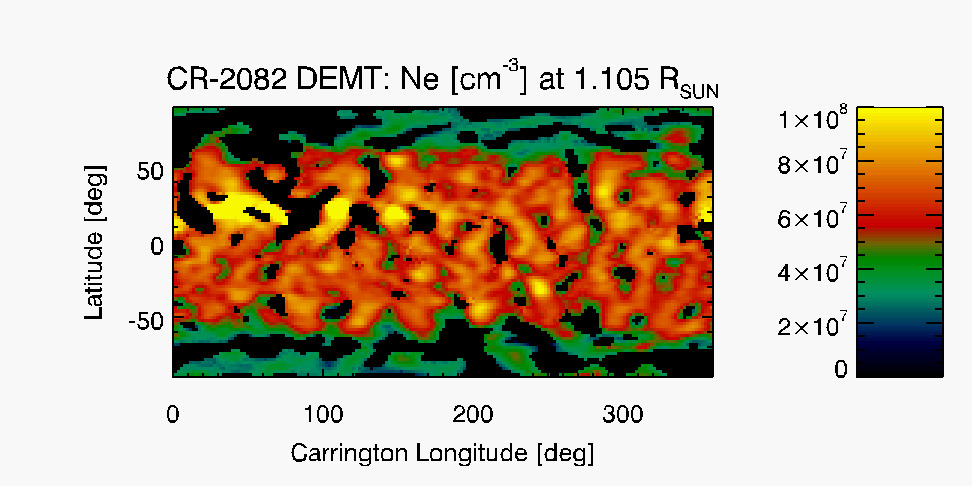
\includegraphics[width=0.4\textwidth,height=0.2\textwidth]{figuras/map_Ne_CR2082_DEMT-EUVI_behind_H1-L3523_r3d_1105_Rsun.jpg}
  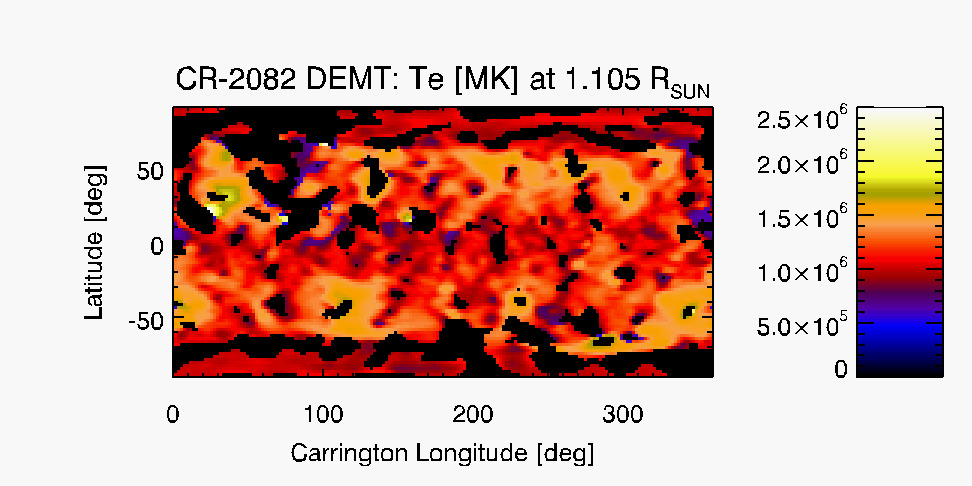
\includegraphics[width=0.4\textwidth]{figuras/map_Tm_CR2082_DEMT-EUVI_behind_H1-L3523_r3d_1105_Rsun.jpg}
  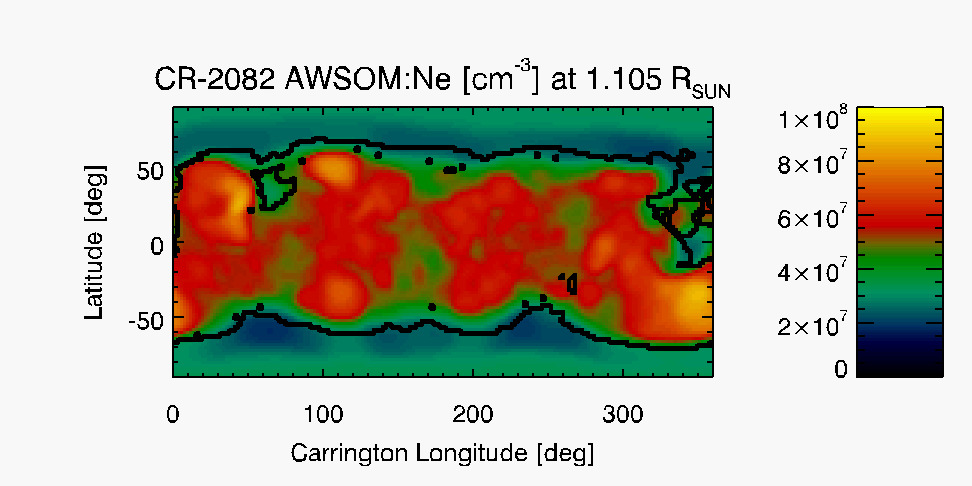
\includegraphics[width=0.4\textwidth]{figuras/map_Ne_awsom_2082_185_short_1105_Rsun.jpg}
  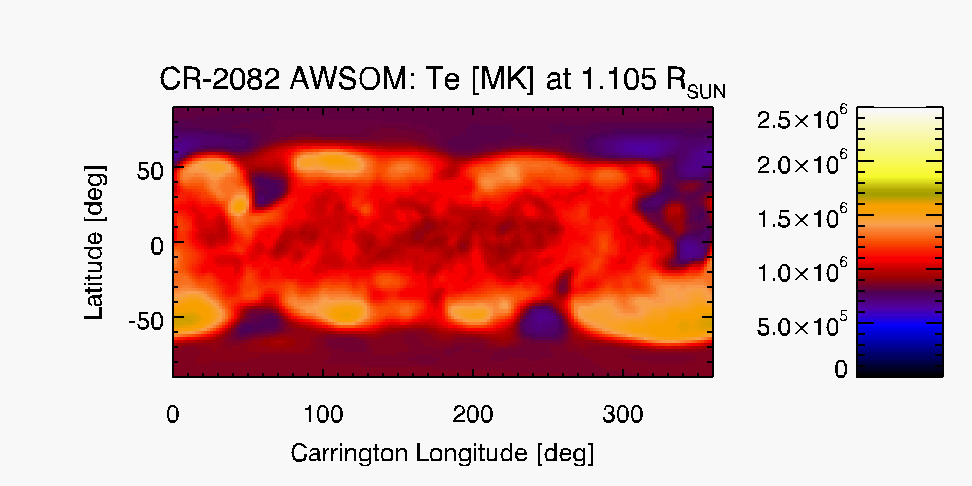
\includegraphics[width=0.4\textwidth]{figuras/map_Te_awsom_2082_185_short_1105_Rsun.jpg}
  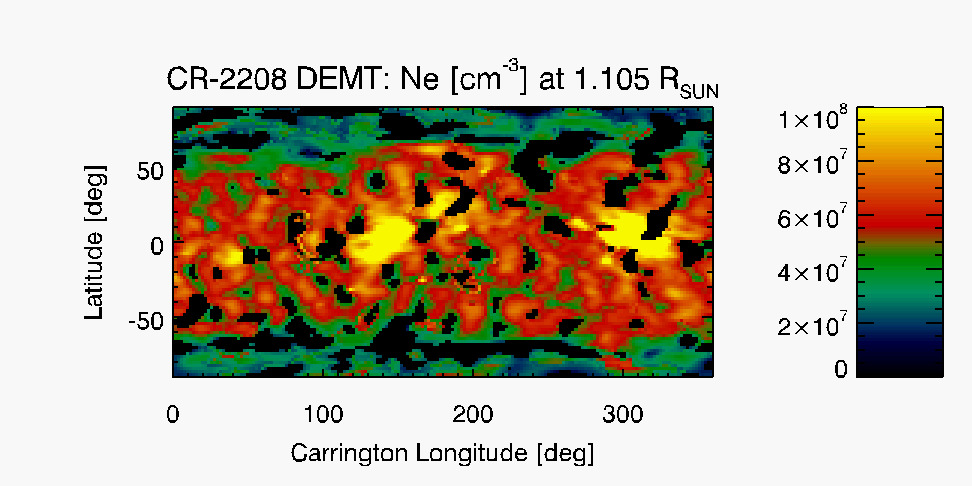
\includegraphics[width=0.4\textwidth]{figuras/map_Ne_CR2208_DEMT-AIA_H1_L522_r3d_1105_Rsun.jpg}
  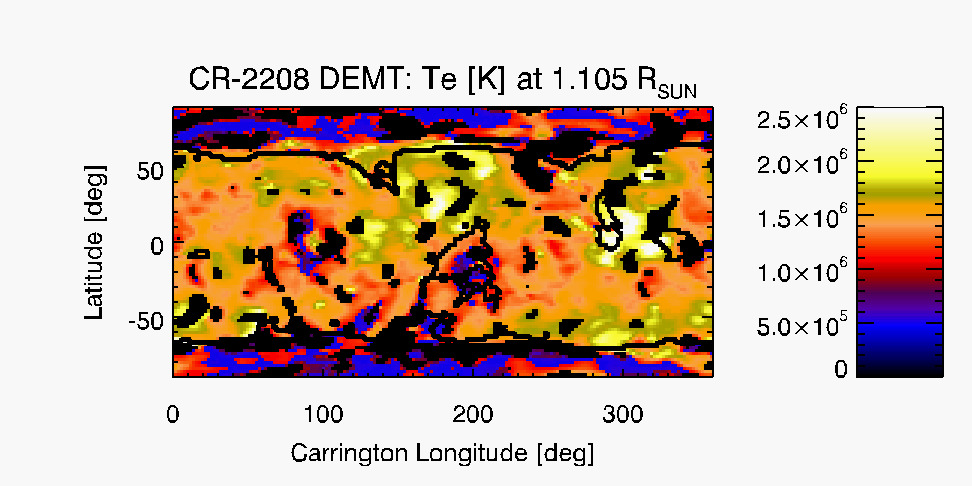
\includegraphics[width=0.4\textwidth]{figuras/map_Tm_CR2208_DEMT-AIA_H1_L522_r3d_1105_Rsun.jpg}  
  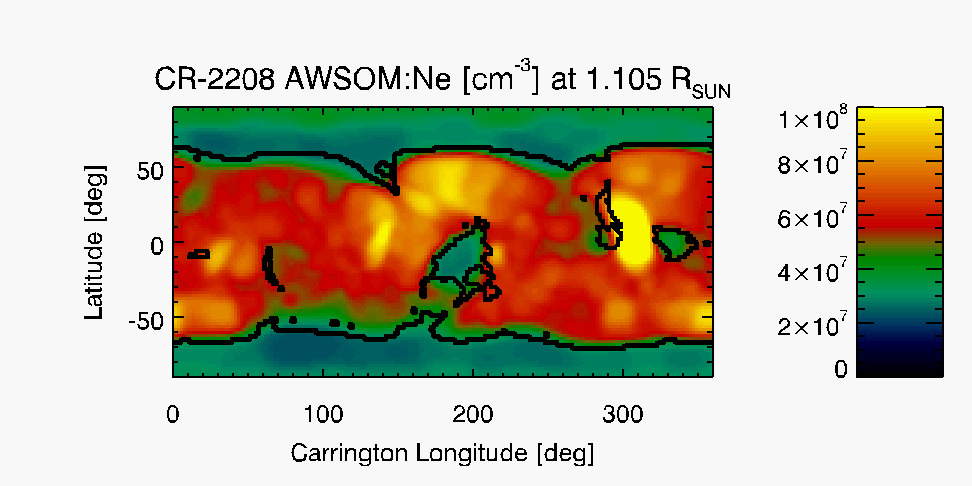
\includegraphics[width=0.4\textwidth]{figuras/map_Ne_awsom_2208_185_short_1105_Rsun.jpg}
  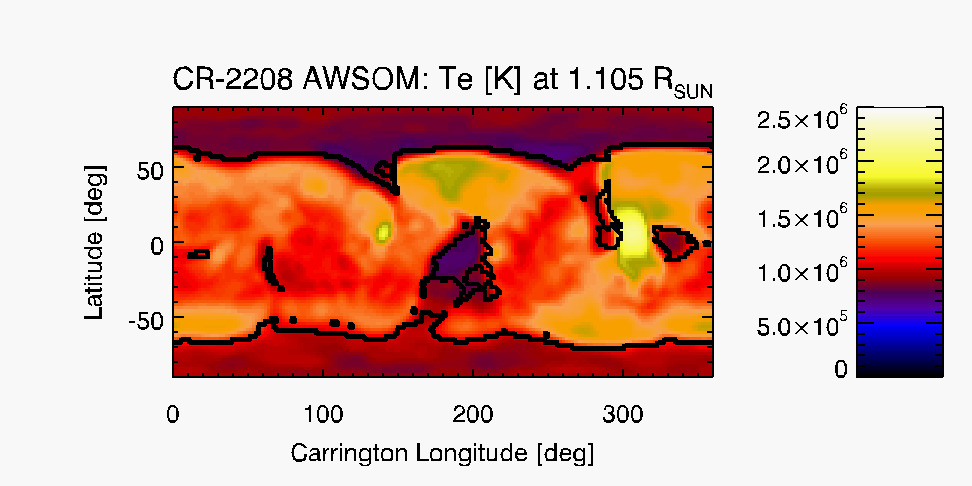
\includegraphics[width=0.4\textwidth]{figuras/map_Te_awsom_2208_185_short_1105_Rsun.jpg}
    \caption{Mapas de Carrington de $T_e$ (derecha) y $N_e$ (izquierda) de CR-2082 y CR-2208 a 1.105 ${\rm R_\odot}$ obtenidas con DEMT y con AWSoM. En los mapas tomográficos, las celdas negras corresponden a regiones no reconstruídas. En todos los paneles las curvas negras indican las fronteras entre las regiones magnéticas abiertas y cerradas (determinadas en base al modelo magnético de AWSoM).}
  \label{fig-carrington}
\end{figure*}


%\begin{figure*}
%  \centering
%  \includegraphics[width=0.4\textwidth]{figuras/Midpoint_2082_demt-proceeding_Rpoint-map.eps}
%  \includegraphics[width=0.4\textwidth]{figuras/Midpoint_2208_demt-proceeding_Rpoint-map.eps}
%  \caption{Lolcalización física de los arcos magnéticos a 1.075 ${\rm R_\odot}$. En amarillo la región cerrada y en violeta la región abierta.}
%  \label{fig-rpoint}
%\end{figure*}

\begin{figure*}
  \centering
  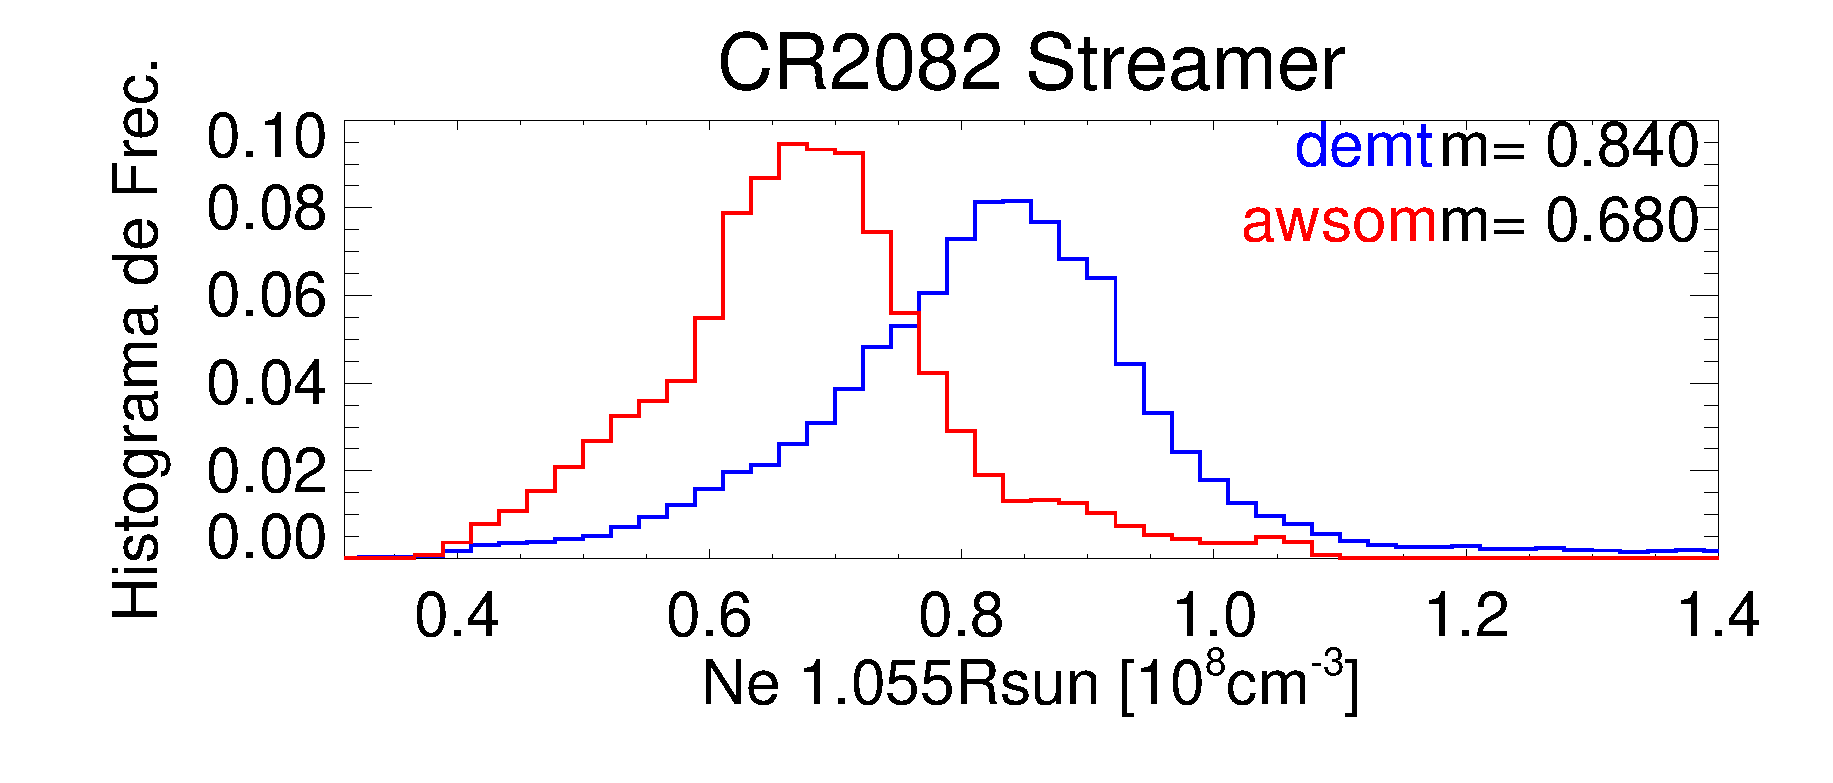
\includegraphics[width=0.32\textwidth]{figuras/proceeding_2082_demt_awsom_streamer_ne_1055.eps}
  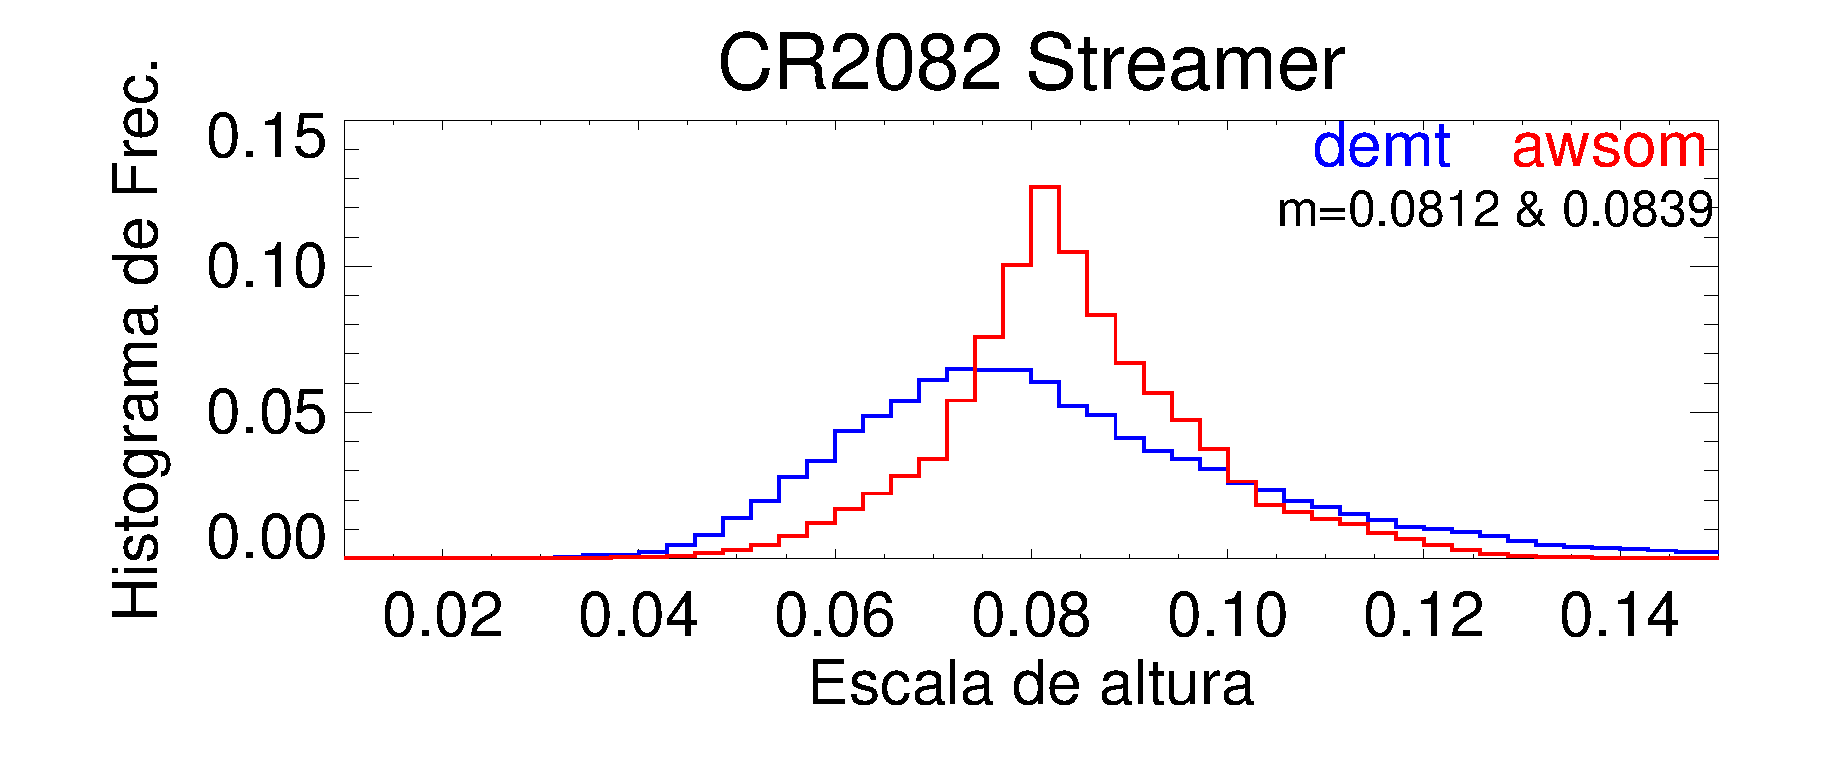
\includegraphics[width=0.32\textwidth]{figuras/proceeding_2082_demt_awsom_streamer_lambda_n.eps}  
  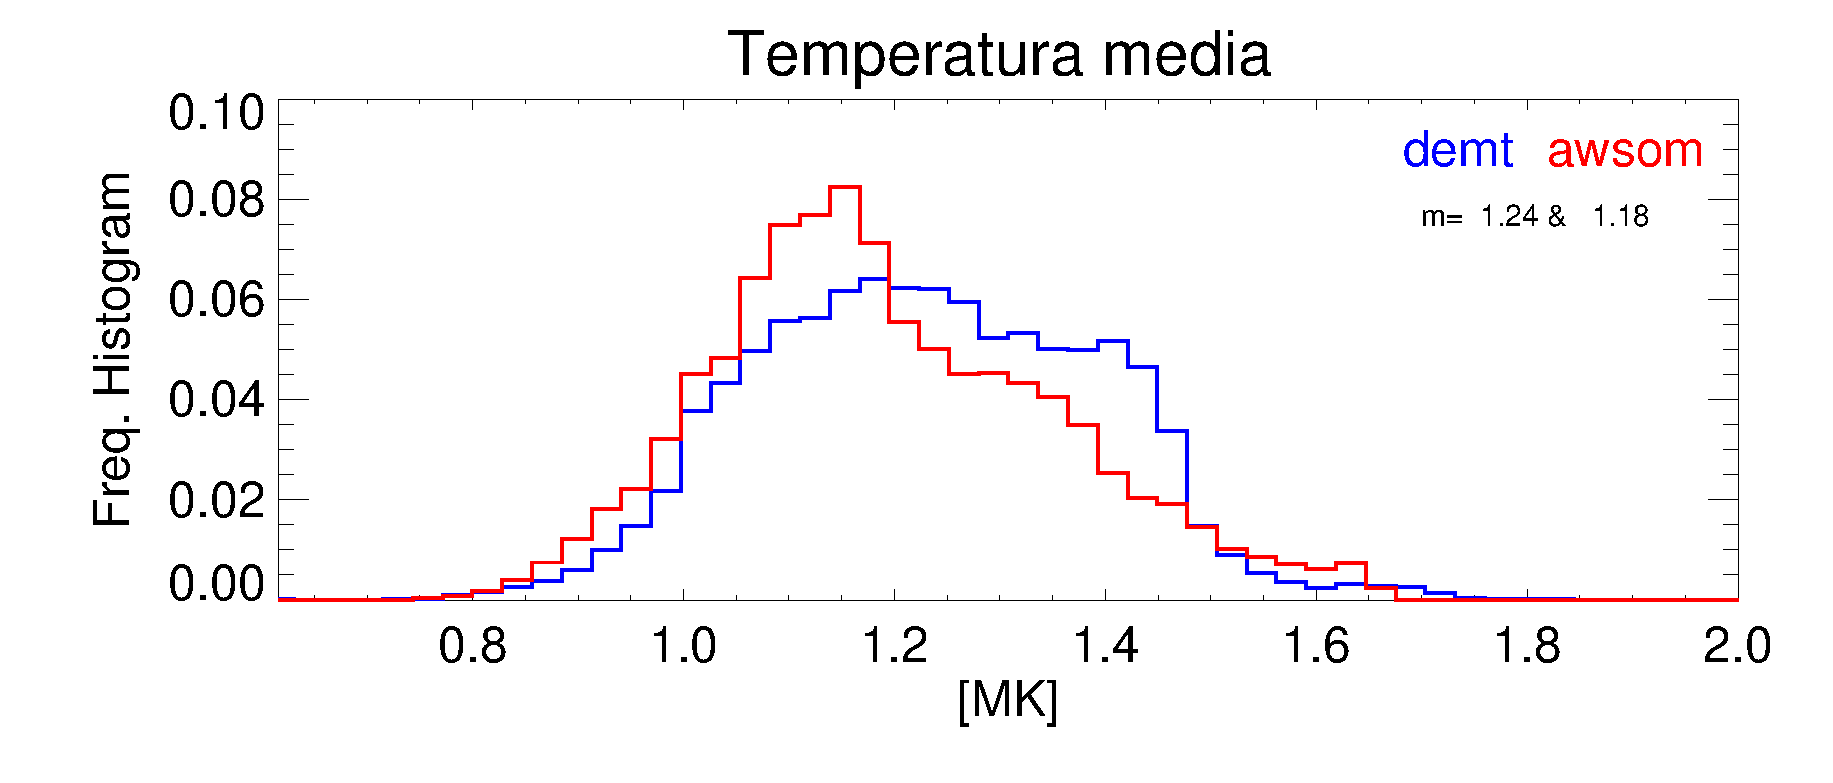
\includegraphics[width=0.32\textwidth]{figuras/proceeding_2082_demt_awsom_streamer_Tm.eps}\\
  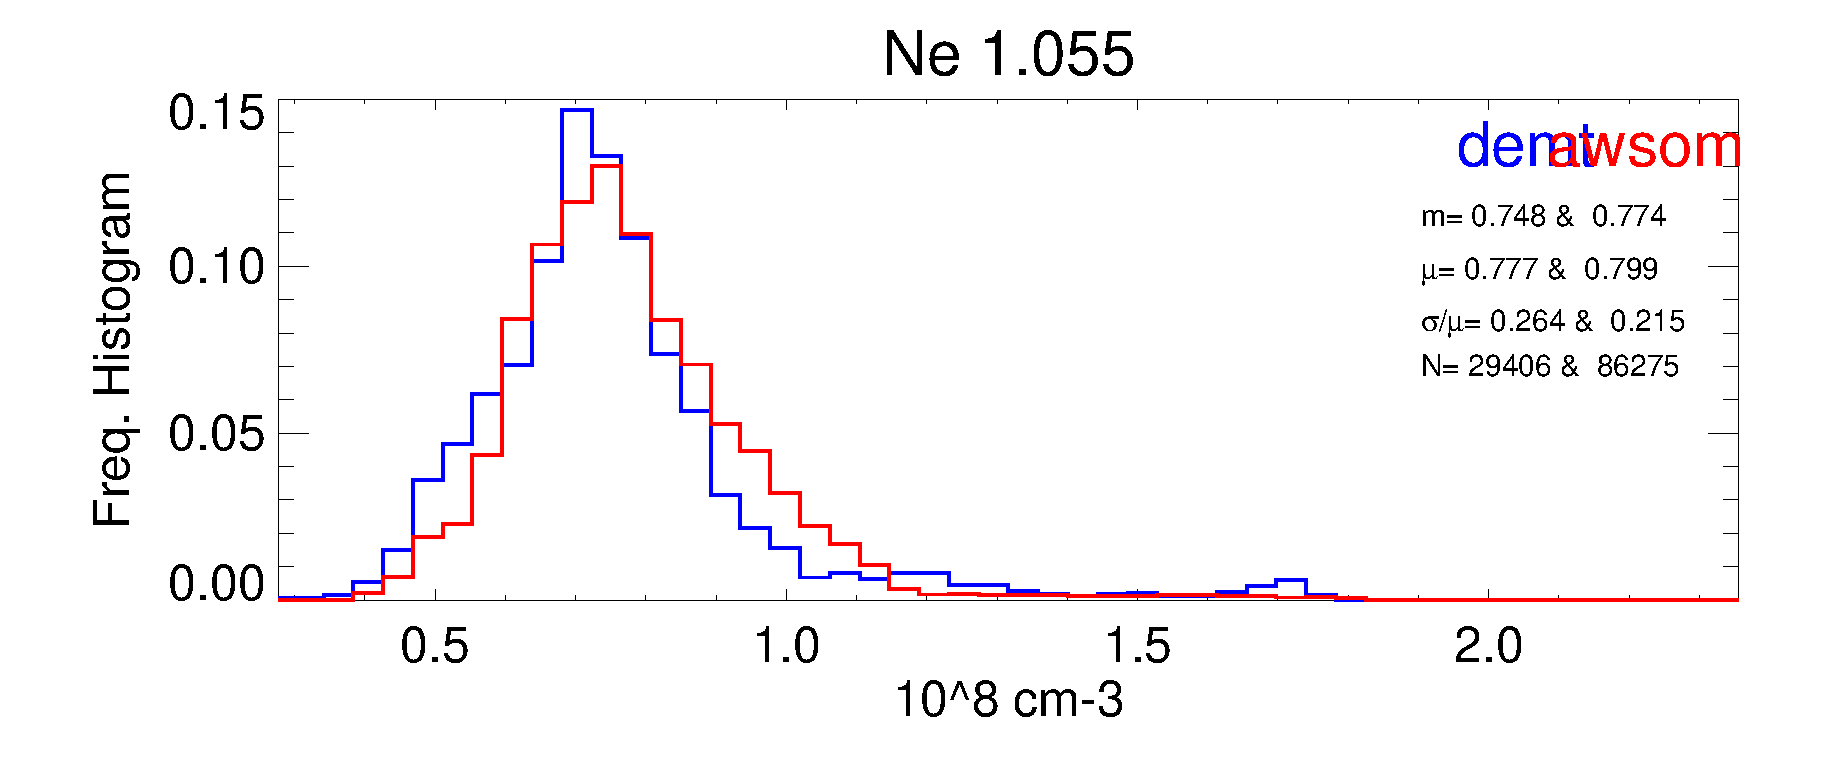
\includegraphics[width=0.32\textwidth]{figuras/proceeding_2208_demt_awsom_streamer_ne_1055.eps}
  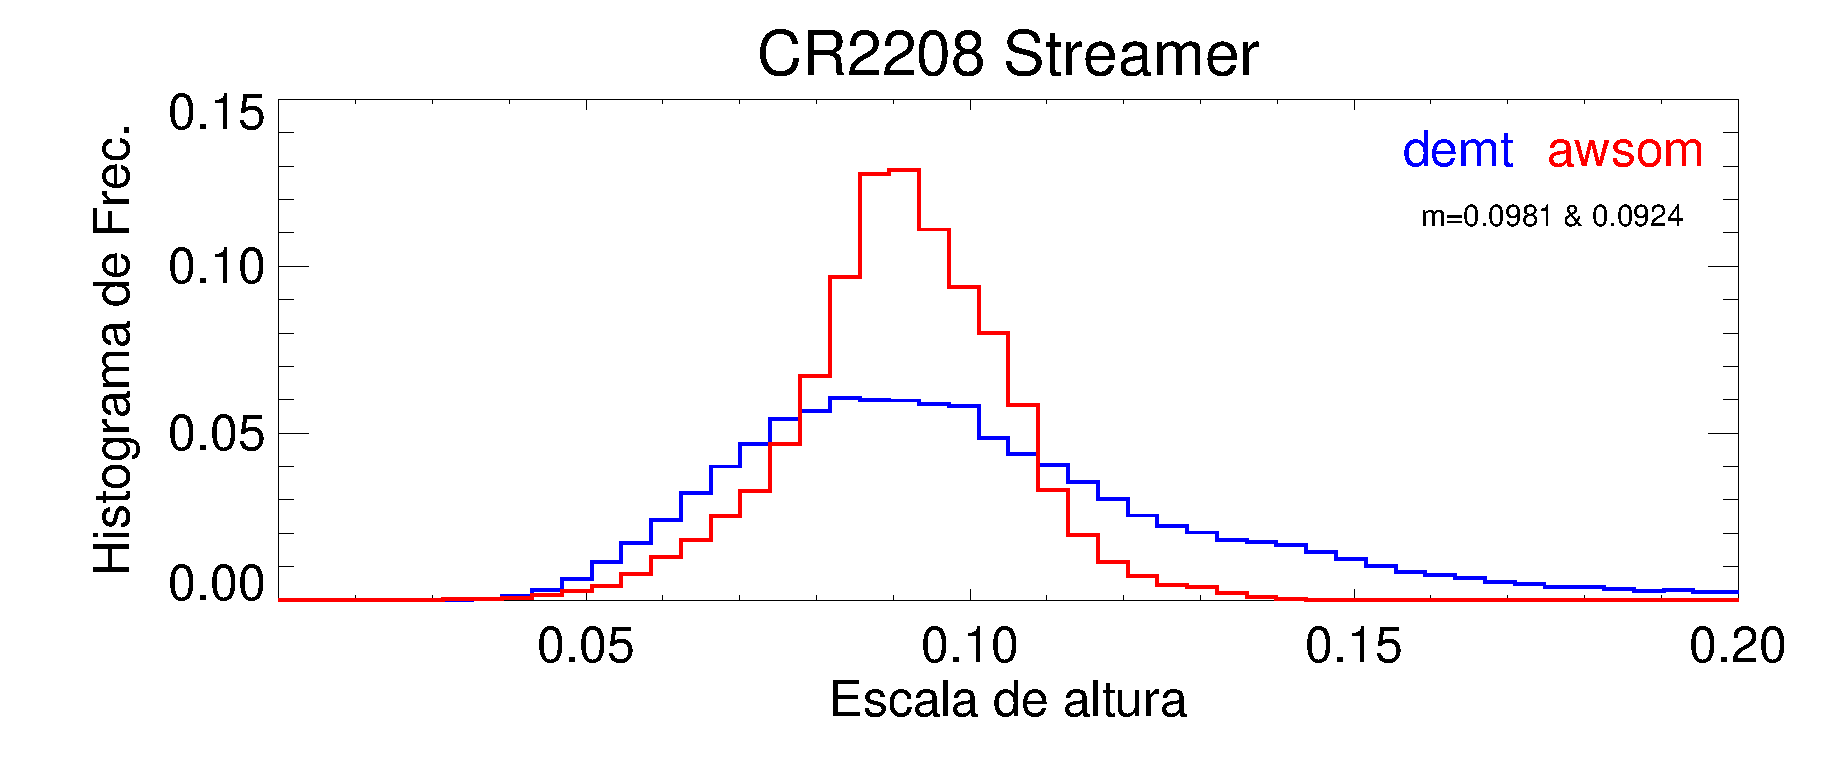
\includegraphics[width=0.32\textwidth]{figuras/proceeding_2208_demt_awsom_streamer_lambda_n.eps}
  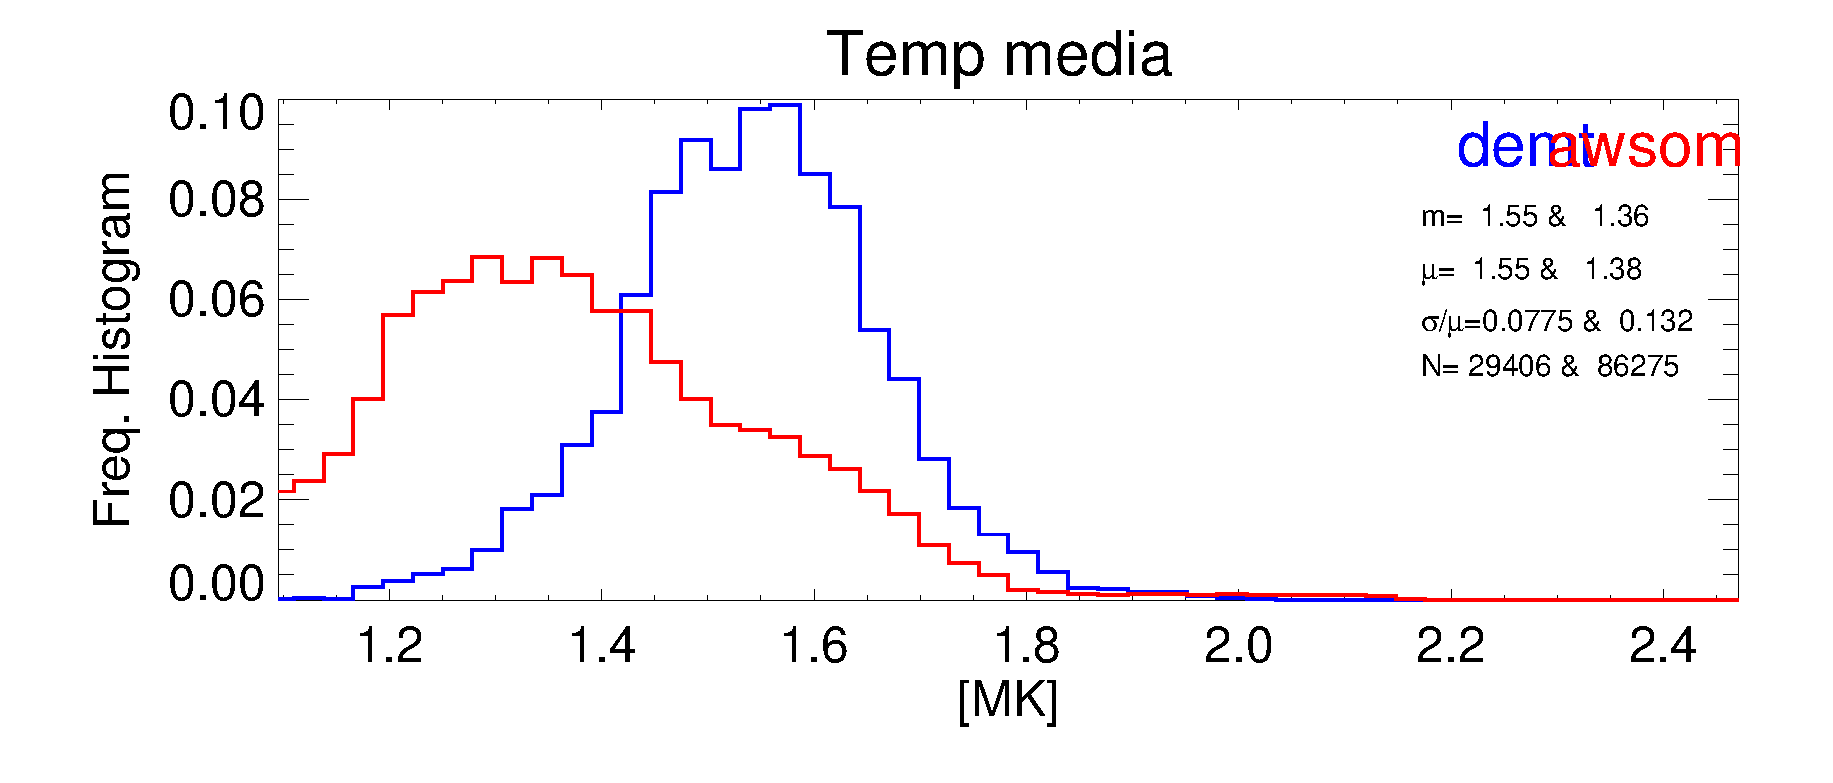
\includegraphics[width=0.32\textwidth]{figuras/proceeding_2208_demt_awsom_streamer_Tm.eps}
%  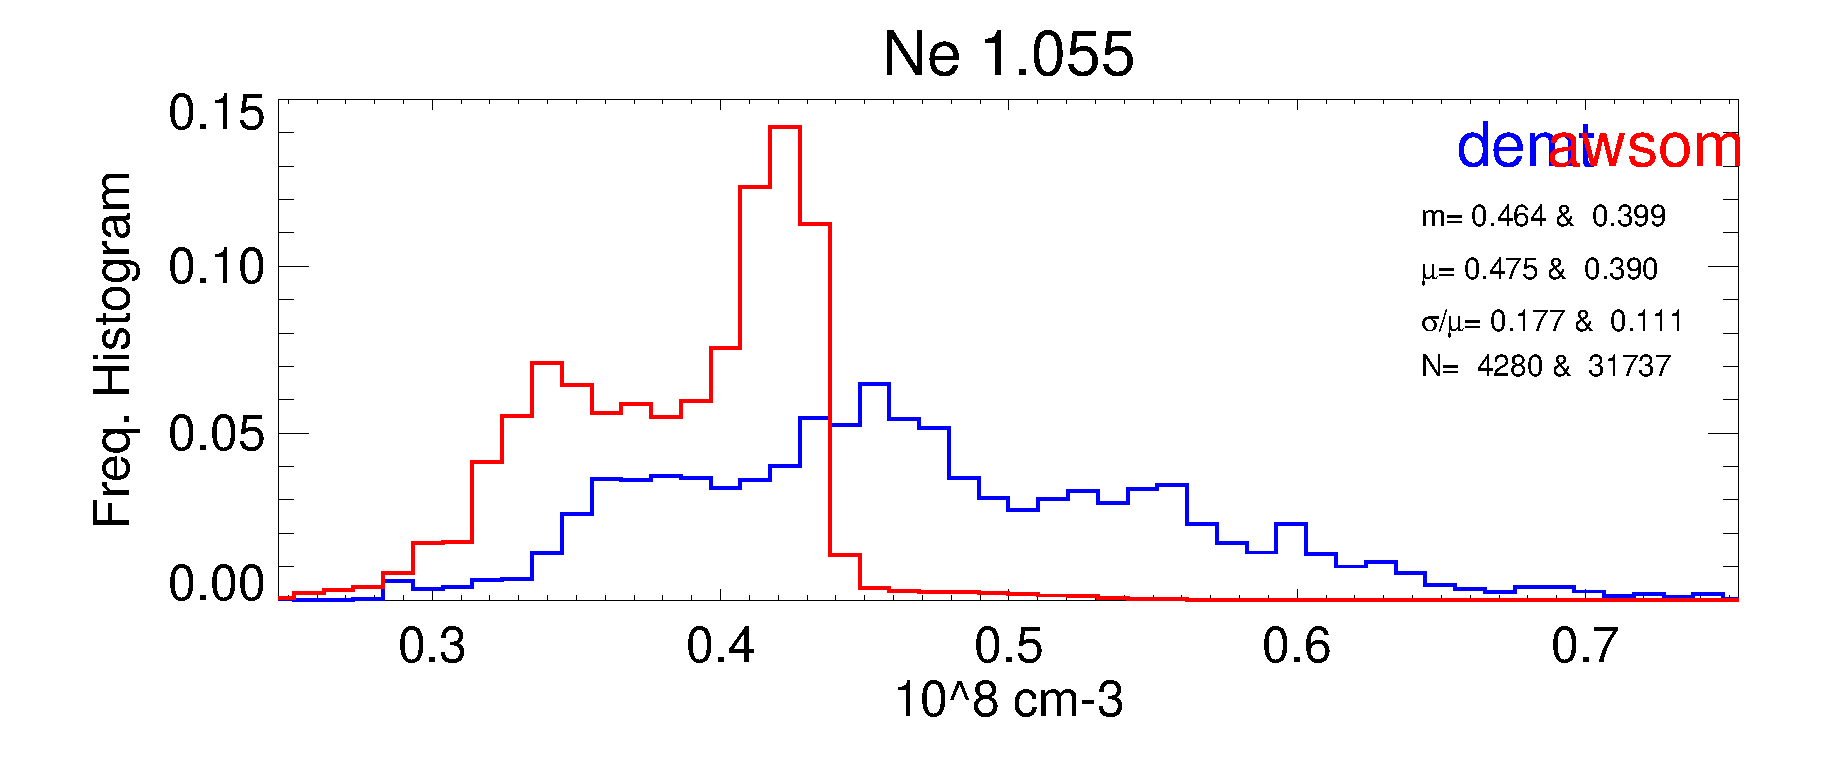
\includegraphics[width=0.32\textwidth]{figuras/proceeding_2082_demt_awsom_CH_ne_1055.eps}
%  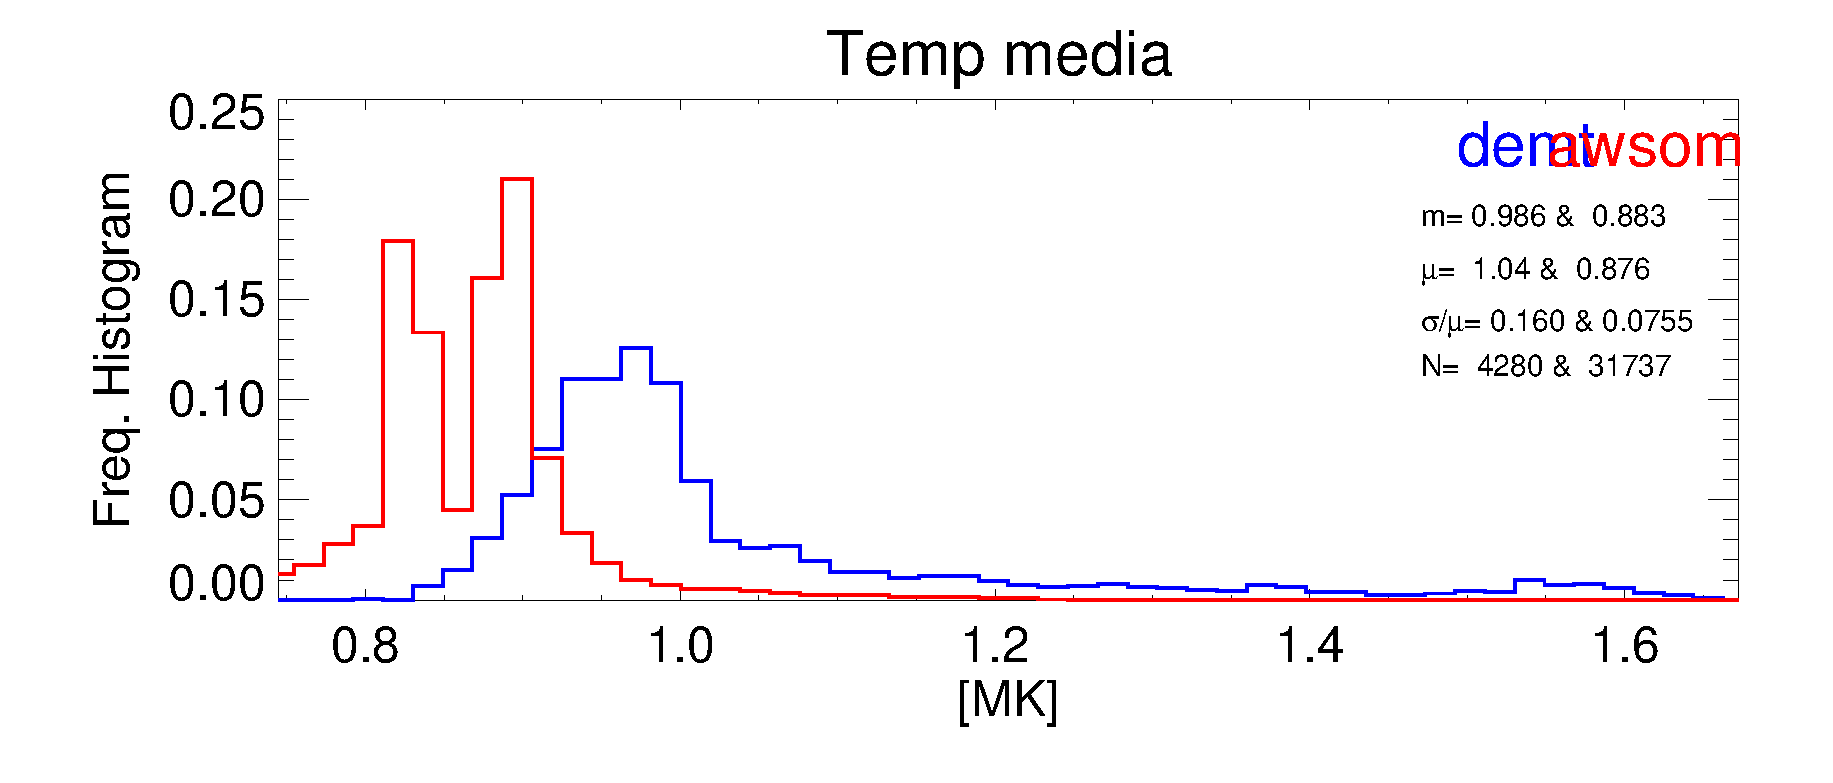
\includegraphics[width=0.32\textwidth]{figuras/proceeding_2082_demt_awsom_CH_Tm.eps}
%  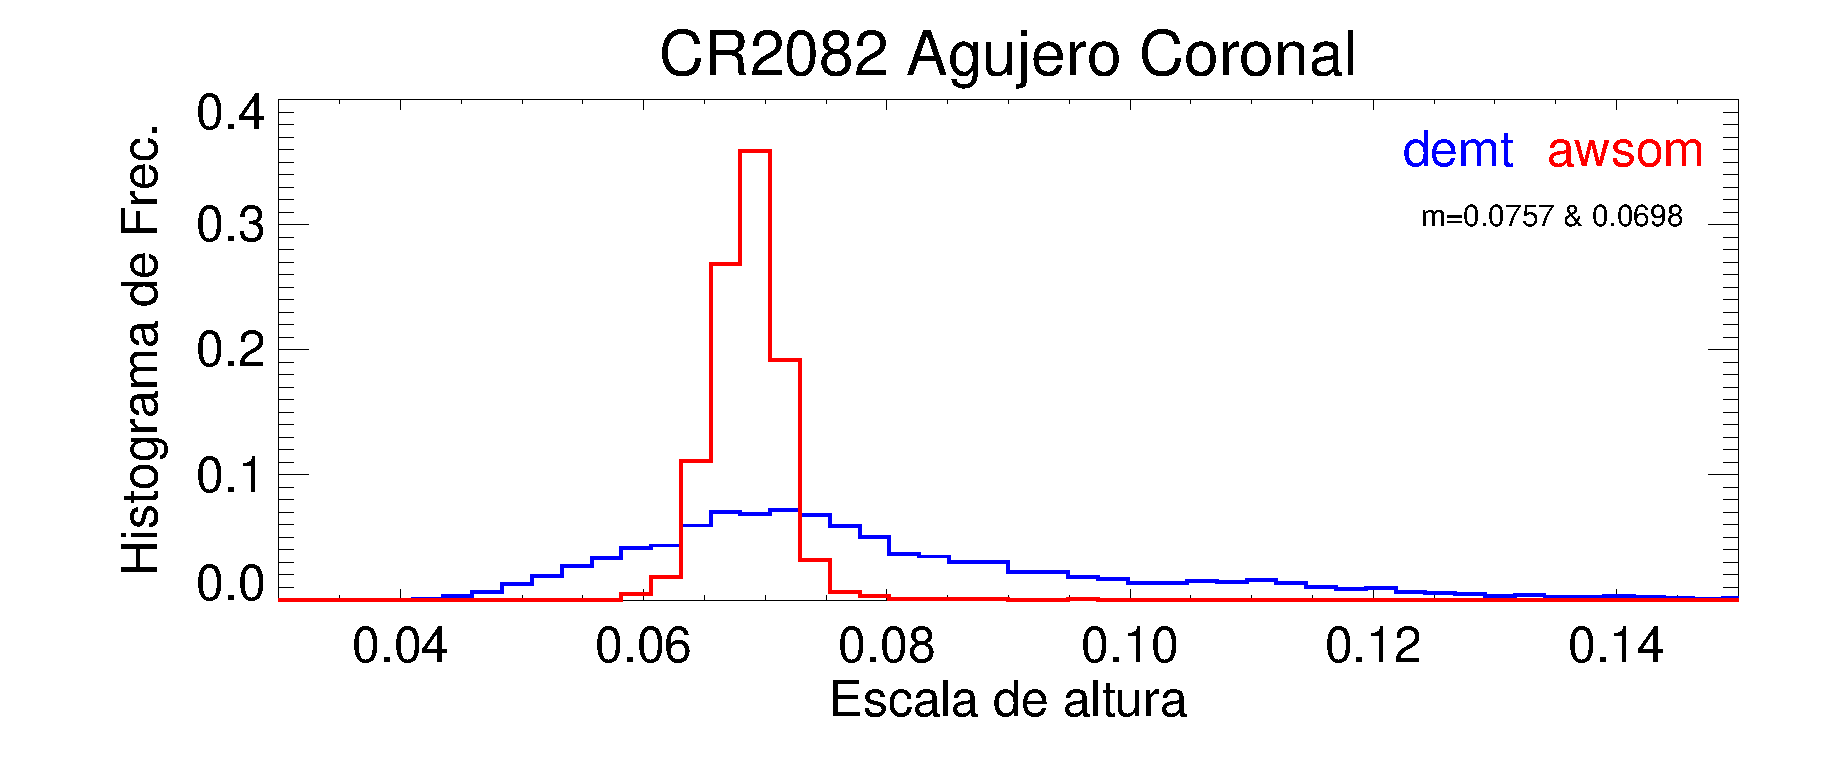
\includegraphics[width=0.32\textwidth]{figuras/proceeding_2082_demt_awsom_CH_lambda_n.eps}\\
%  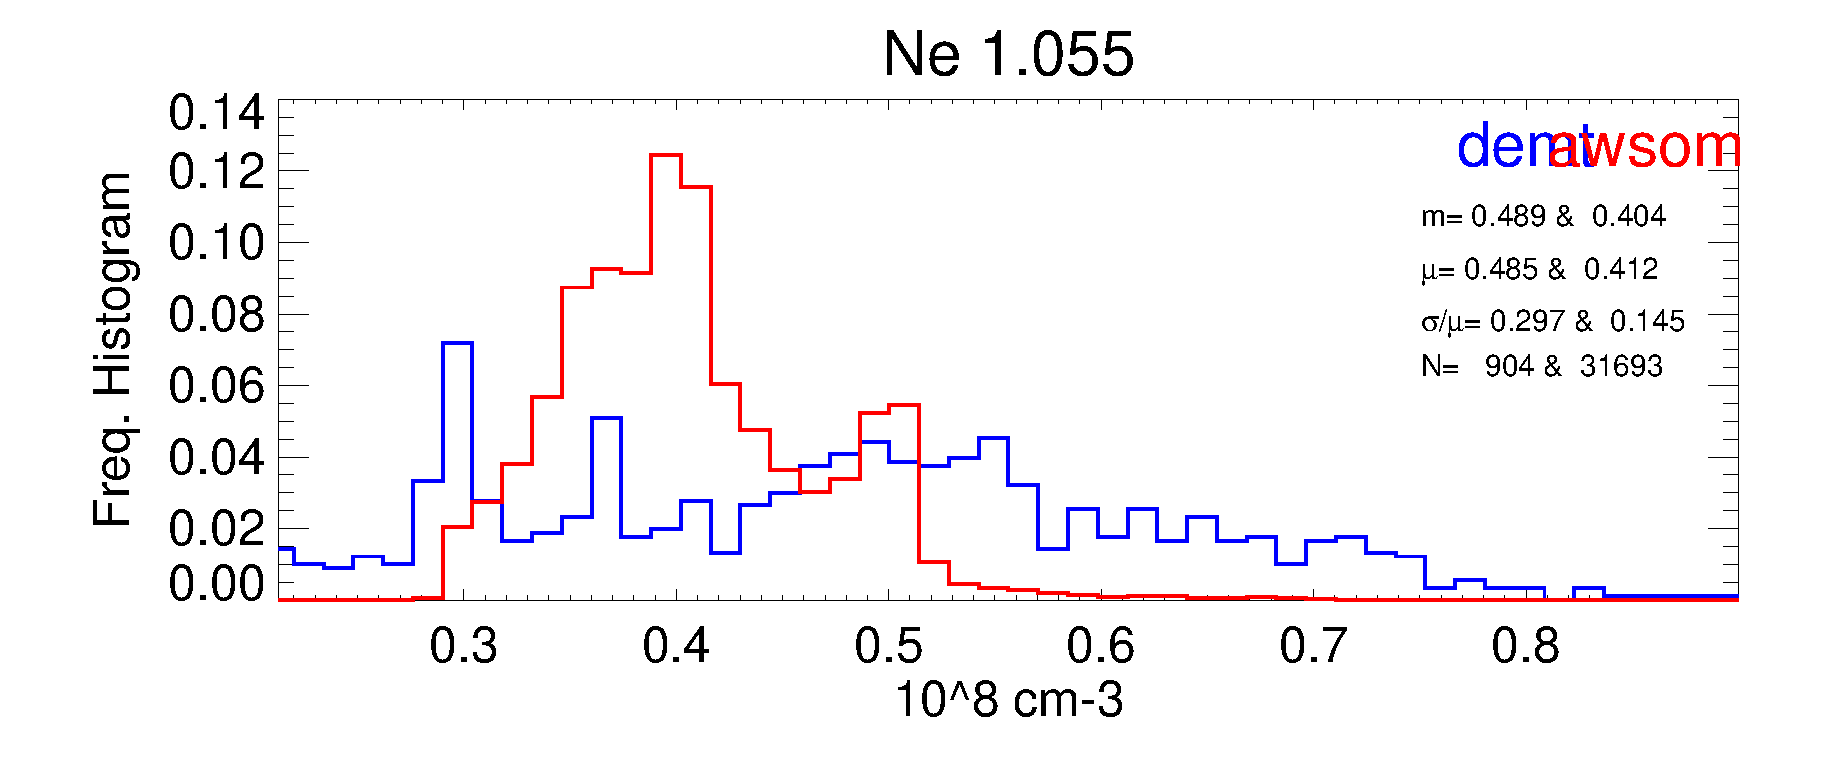
\includegraphics[width=0.32\textwidth]{figuras/proceeding_2208_demt_awsom_CH_ne_1055.eps}
%  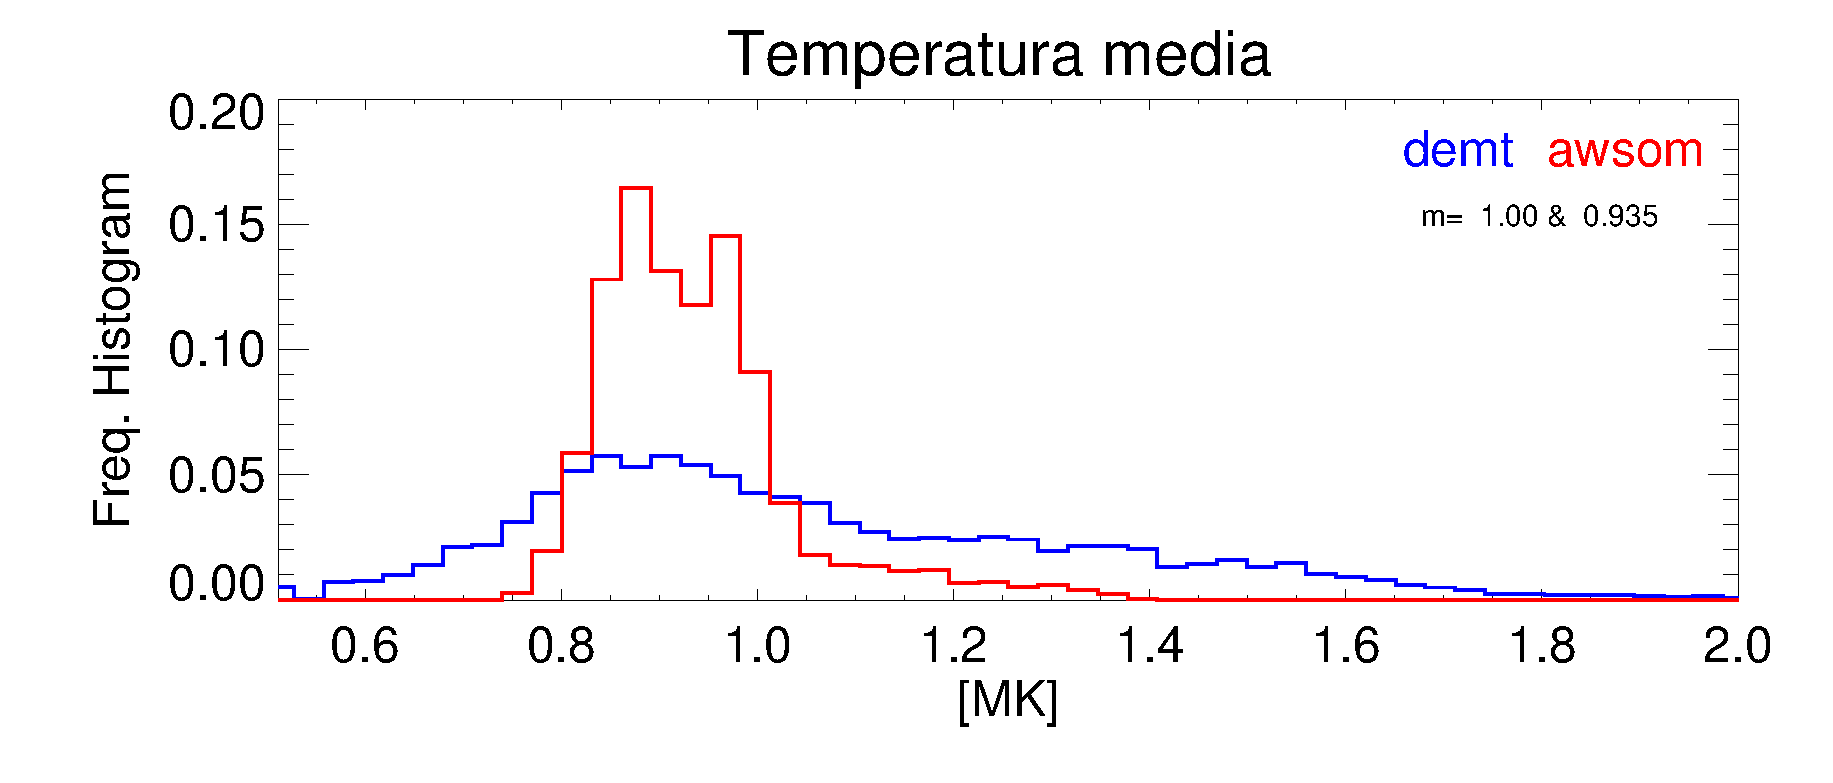
\includegraphics[width=0.32\textwidth]{figuras/proceeding_2208_demt_awsom_CH_Tm.eps}
%  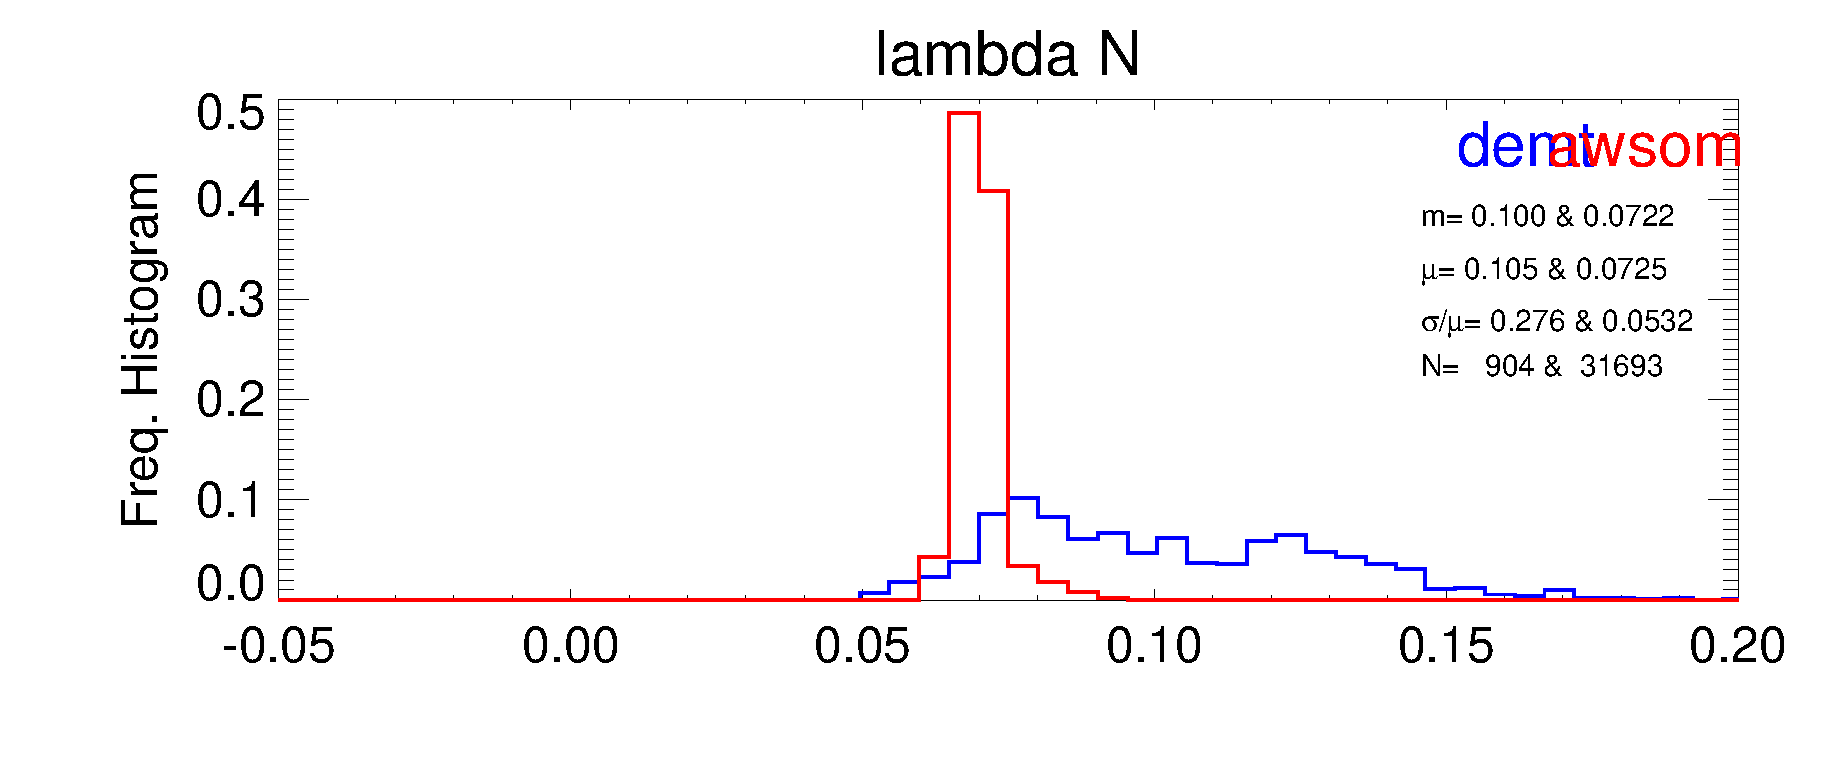
\includegraphics[width=0.32\textwidth]{figuras/proceeding_2208_demt_awsom_CH_lambda_n.eps}
  \caption{Histograma de frecuencia de CR-2082 y CR-2208 de $N_e$ a 1.055 ${\rm R_\odot}$, escala de altura de la densidad electrónica y $\left<T_e\right>$. En azul se muestran los resultados obtenidos con DEMT y en rojo con AWSoM junto con la mediana de la respectiva estadística para la región del streamer.}
  \label{fig-histos}
\end{figure*}

%\begin{figure*}
%  \centering
%  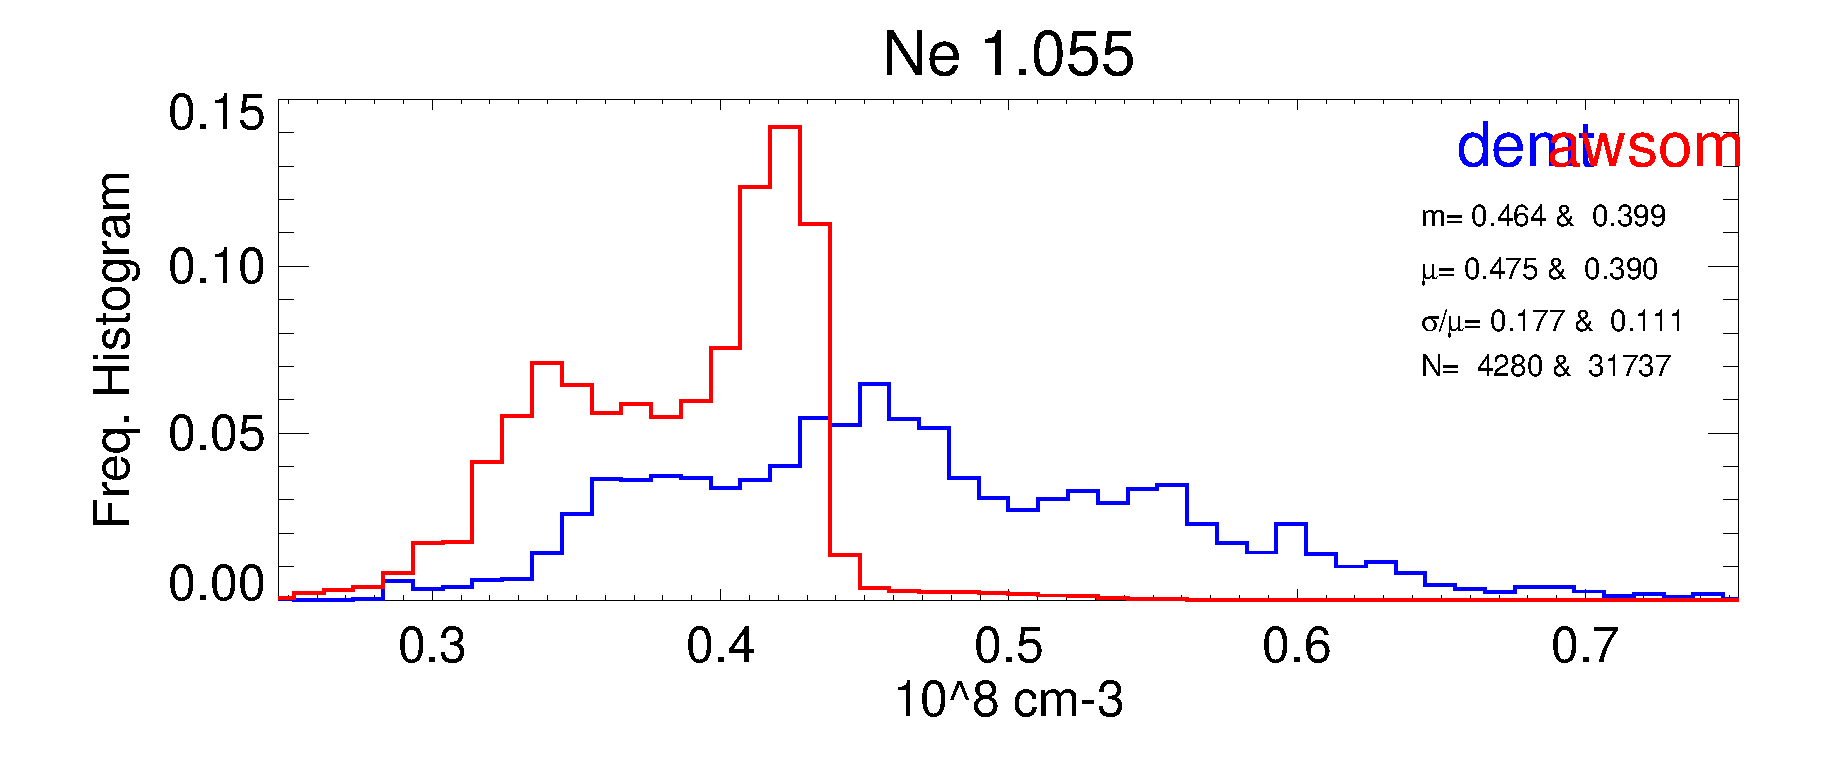
\includegraphics[width=0.32\textwidth]{figuras/proceeding_2082_demt_awsom_CH_ne_1055.eps}
%  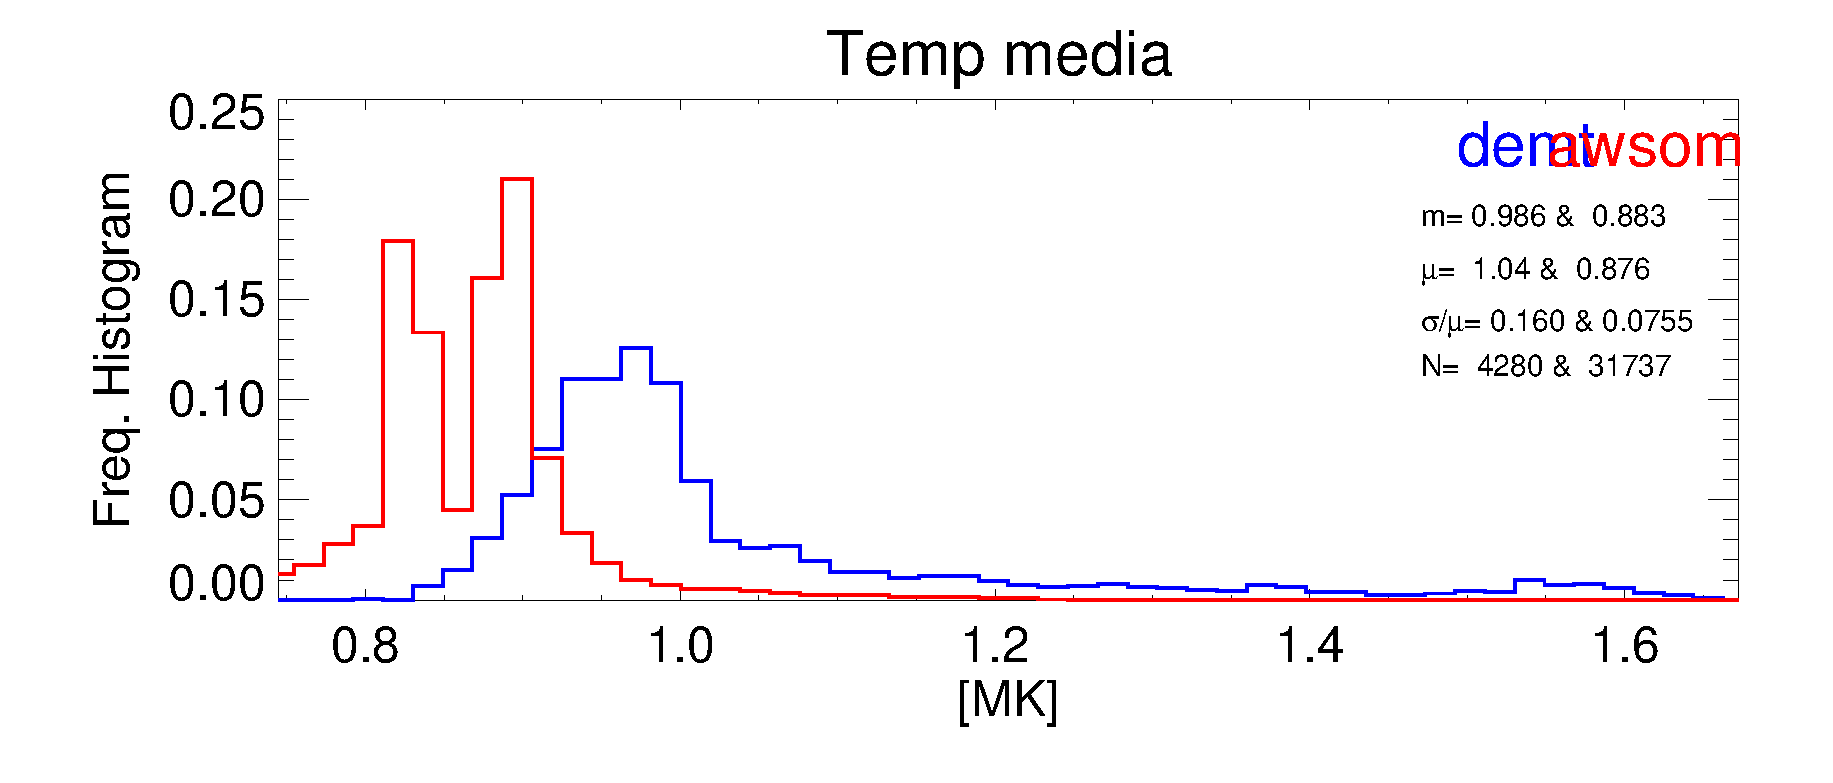
\includegraphics[width=0.32\textwidth]{figuras/proceeding_2082_demt_awsom_CH_Tm.eps}
%  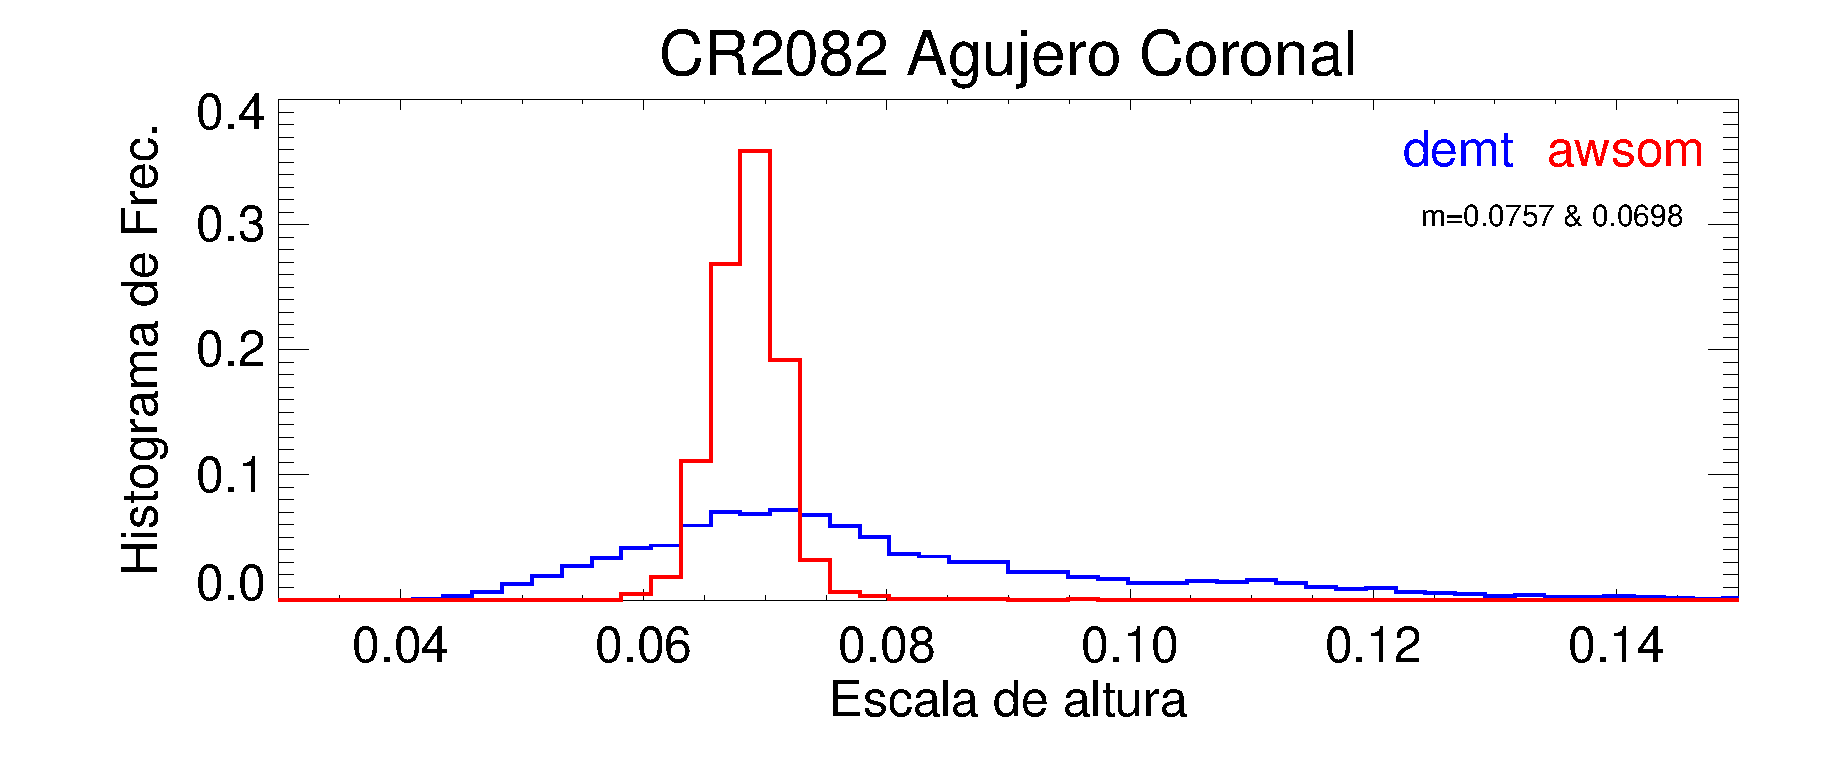
\includegraphics[width=0.32\textwidth]{figuras/proceeding_2082_demt_awsom_CH_lambda_n.eps}\\
%  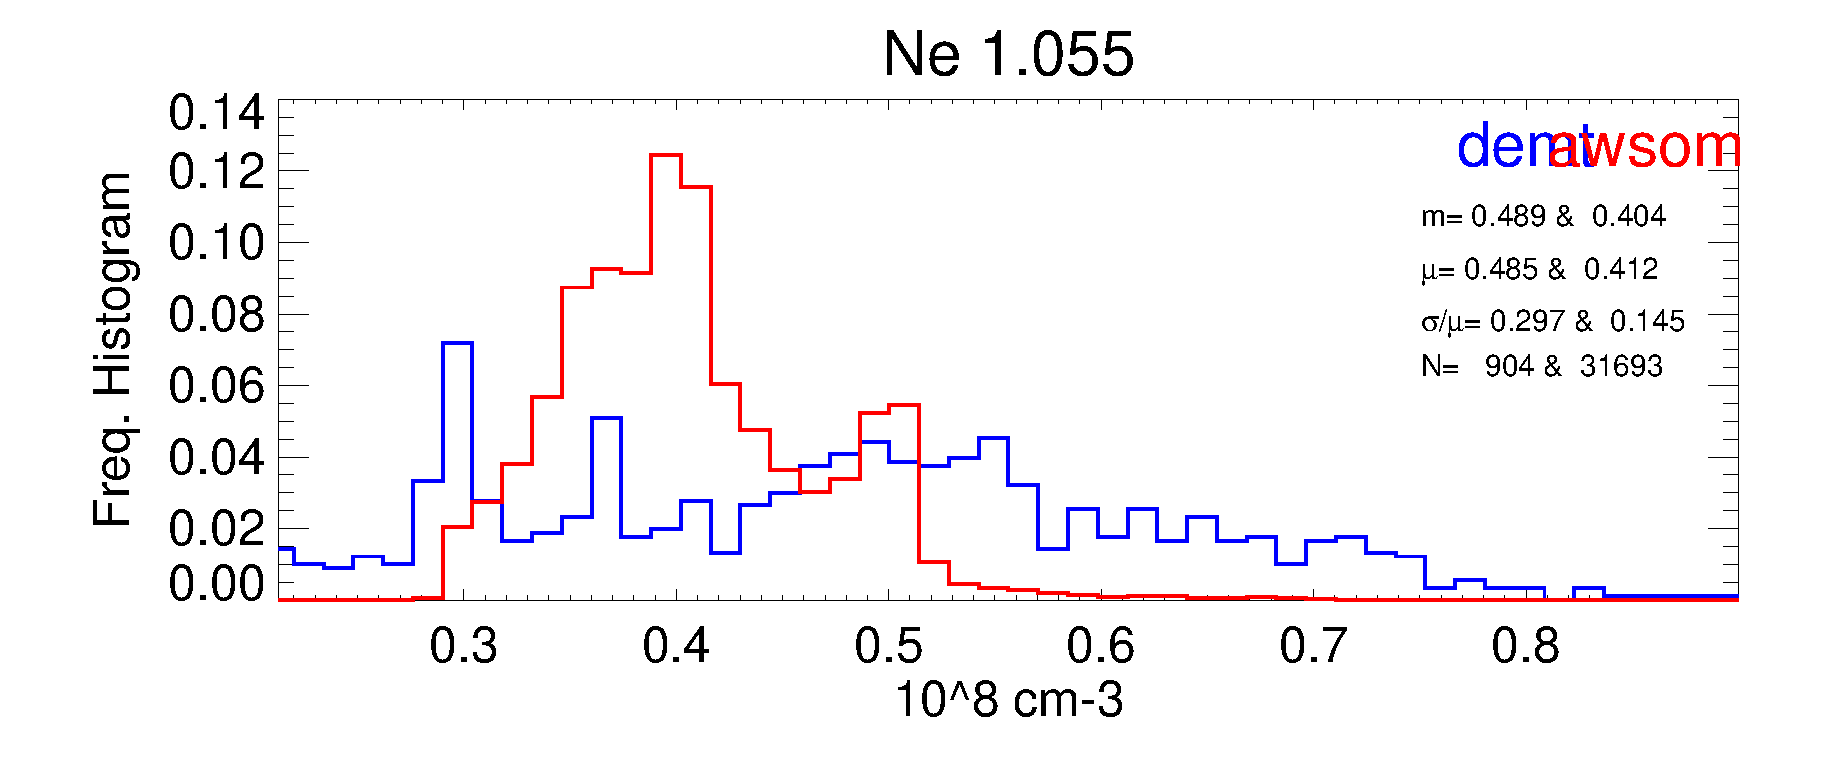
\includegraphics[width=0.32\textwidth]{figuras/proceeding_2208_demt_awsom_CH_ne_1055.eps}
%  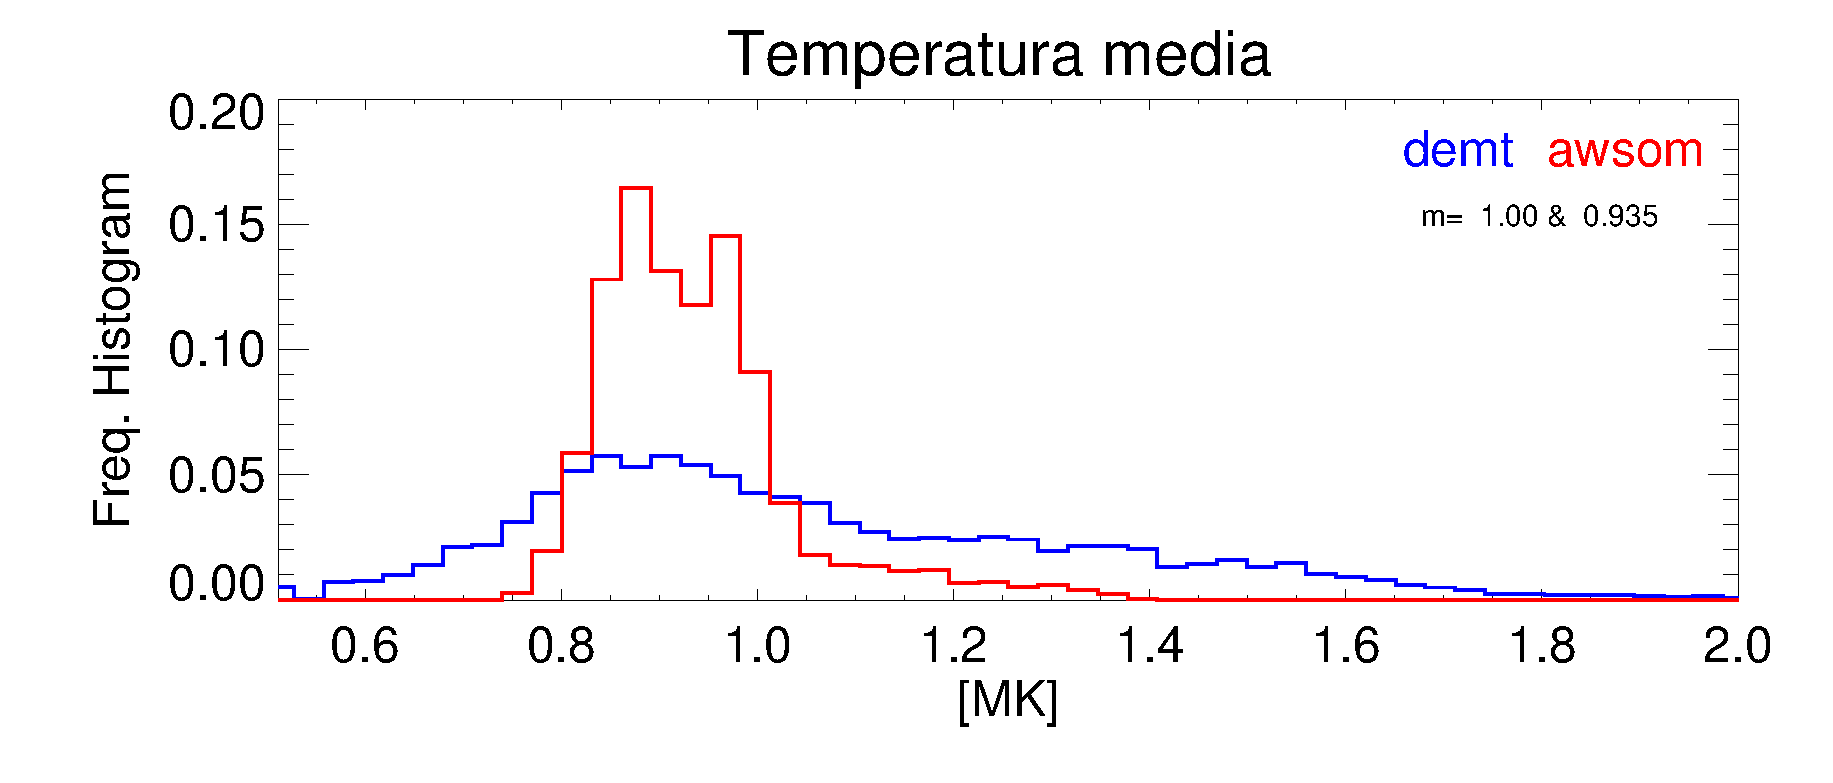
\includegraphics[width=0.32\textwidth]{figuras/proceeding_2208_demt_awsom_CH_Tm.eps}
%  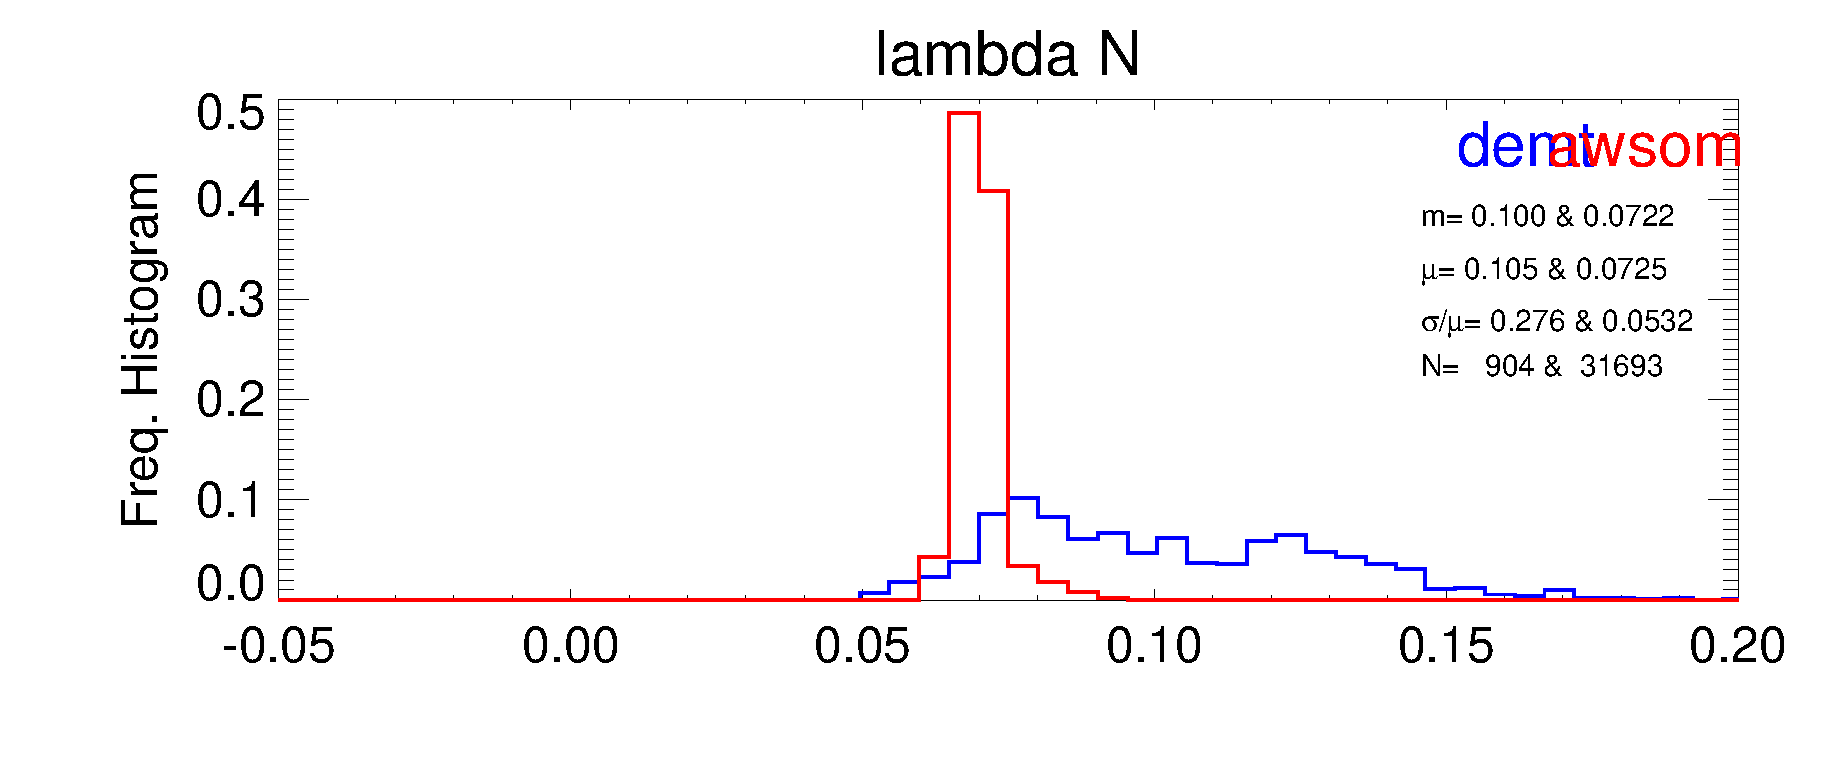
\includegraphics[width=0.32\textwidth]{figuras/proceeding_2208_demt_awsom_CH_lambda_n.eps}
%  \caption{Histogramas}
%  \label{fig-histos2}
%\end{figure*}

\section{Discusión y trabajo futuro}

El modelo AWSoM reproduce la simetría axial de las estructuras de streamer y agujero coronal de forma global. Es capaz de reproducir las estructuras magnéticas con temperatura creciente. Para estas estructuras se observan diferencias de la temperatura media menores al 30\%. Los ajustes en densidad presentan escalas de altura $\lambda_n$ muy similares y diferencias en la densidad basal $N_e(r=1.05\,{\rm R_\odot})$  menores al 30 \% según la rotación modelada y es capaz de reproducir temperaturas crecientes en las estructuras magnéticas con una diferencia $<30 \%$. 
 
%Este anális muestra un gran avance en la capacidad del modelo para reproducir la termodinámica de la baja corona. De todas formas un enfoque diferente en la conversión de modos de Alfvén en la región de transición podría generar arcos con temperaturas decrecientes. Este tipo de arcos son dominantes en la zona proxima al ecuador duranto un mínimo de actividad solar \citep{nuevo_2013}.

El análisis presentado en este trabajo muestra un  avance en la capacidad del modelo AWSoM para reproducir la termodinámica de la baja corona descripta por la técnica DEMT. Sin embargo, el modelo no logra reproducir arcos con temperaturas decrecientes, que son dominantes en la zona próxima al ecuador durante el mínimo de actividad solar \citep{nuevo_2013}.  La incorporación de la conversión de modos de Alfvén en modos compresibles podría permitir que el modelo reproduzca estas estructuras \citep{schiff_2016}.

Próximamente se publicará una comparación más extensa y detallada de las cantidades termodinámicas y energéticas derivadas de DEMT y el modelo AWSoM para estas dos rotaciones considerando subregiones del streamer y los agujeros coronales.

%\begin{acknowledgement}
%\texttt{Al Mate Misionero}
%\end{acknowledgement}

%%%%%%%%%%%%%%%%%%%%%%%%%%%%%%%%%%%%%%%%%%%%%%%%%%%%%%%%%%%%%%%%%%%%%%%%%%%%%%
%                                                                            %
%  Por favor no modifique las líneas de la bibliografía, salvo el nombre     %
%  el archivo de Bibtex con la lista de citas (sin la extensión .BIB)        %
%                                                                            %
%  Please do not modify the following lines, except the name of the Bibtex   %
%  file (whithout the .BIB extension)                                        %
%                                                                            %
%%%%%%%%%%%%%%%%%%%%%%%%%%%%%%%%%%%%%%%%%%%%%%%%%%%%%%%%%%%%%%%%%%%%%%%%%%%%%% 

\bibliographystyle{baaa}
\small
\bibliography{baaa61b_2020_dglloveras}
 
\end{document}
